\PassOptionsToPackage{hyphens}{url}

\documentclass[12pt]{article}
%\documentclass[12pt, executivepaper]{article}
% \documentclass[12pt,twocolumn]{article}

\usepackage[title]{appendix}
\usepackage{graphicx} % need this package
\usepackage{hyperref}
\usepackage{listings}
\usepackage{mathtools}
\DeclarePairedDelimiter\ceil{\lceil}{\rceil}
\DeclarePairedDelimiter\floor{\lfloor}{\rfloor}


\begin{document}
\title{How to Seek: An Exploration of Pursuit Methods in Games\thanks{Great thanks and praise is given to the wonderful mentorship and advisement of Dr. Diane Pozefsky at the University of North Carolina at Chapel Hill.}}
\author{Taylor Smith 
\\
University of North Carolina at Chapel Hill		
}
\date{24 April 2020}
\maketitle
\begin{abstract}
This paper explores the problem of \textbf{pursuit-evasion} through the construction and comparison of three different approaches to seeking. One, denoted the Corner- and Room-Based Model, attempts to approximate human-like behavior. Two other Graph-Based Models provide benchmark comparisons against which to compare this deterministic finite automation based model. A common experimental environment is set up and used to compare these different models.
\end{abstract}

\section{Introduction}
Hide and Seek is a well-known, classic children's game where one or multiple player(s), designated ``Seeker(s),'' try to find one or more other players, called ``Hider(s).'' This game is easily conceptualized and solved by human agents, who can conceive of real-world spaces and areas as potential hiding spots and are psychologically built to navigate the world around them. A significant and non-trivial problem in artificial intelligence (AI) is teaching a computer agent to perform the same actions.

The OpenAI team, known for such innovative work as OpenAI Five, the AI team that can beat world-class players in the competitive five-on-five strategy video game \textit{Dota 2}, explored a multi-agent version of Hide and Seek\cite{BakerPaper,OpenAI}. Their research deployed a reinforcement algorithm on agents which could grab and lock objects and see using a ``lidar-like sensor.'' Training the agents resulted in several different strategies, including the hiders building shelters, the seekers using ramps, and, amazingly, the seekers ``surfing'' on blocks. Their paper and its corresponding article demonstrate that a reinforcement algorithm at scale can produce multiple agents which utilize complex tools and even coordinate. While learning strategies, the two-sided environment creates pressures for the opposing team to react and produce counter-strategies. The paper concludes that ``multi-agent competition may scale better with increasing environment complexity and leads to behavior that centers around far more human-relevant skills than other self-supervised reinforcement learning methods such as intrinsic motivation.'' As with the team's other work, this paper provides a benchmark in the evolution of artificial intelligence, prompting us to think deeply about the nature of the problem and whether it may be suitable to all games and uses. Are there approaches other than a multi-agent-competition-based reinforcement algorithm? If so, what are they, and how well do they work?

\subsection{Artificial Intelligence}
In games, artificial intelligence generates ``responsive, adaptive, or intelligent behaviors primarily in non-player characters similar to human-like intelligence''\cite{AIDef}. Unlike machine learning, AI in games serves to improve the game-player experience. Since games take place in an environment where the computer has the ability to know everything about the player state, producing behavior of the opponent that approximates intelligence (or, perhaps sometimes, stupidity) is a non-trivial matter. This challenge applies through many examples, including developing behavior for another poker player, a ghost in Pac-Man, or an enemy soldier in a First-Person Shooter. For a given problem, there are multiple approaches, including deterministic methods, various algorithms, learning techniques, and more. Some games require numerous difficulty levels, which induces different approaches and solutions. 
The goal of this project will be to explore these approaches as they relate to the problem of \textbf{Seeking}, also known as Pursuit-Evasion, and run automated experiments to compare their success. Different parameters will be explored, including how the seeker sees, how it moves (e.g. should the agent move to where it saw the hider? Should it attempt to guess where it will move?), and the algorithm which governs its choices and decisions.

\subsection{What is Seeking?}
Seeking is identified in the formal literature as \textbf{pursuit-evasion}, variants of which are known as \textbf{cops and robbers} and \textbf{graph searching}. Pursuit-Evasion formally defines the problem of one group attempting to track down members of another group within an environment. One subset of these problems uses a graph to model the environment (these sub-problems are formally called \textbf{discrete pursuit-evasion} or \textbf{graph searching}), and another models the environment in a continuous and geometric fashion (formally and fittingly called \textbf{continuous pursuit-evasion}). 

The original work on pursuit-evasion was explored by Dr. Rufus Isaacs in his book \textit{Differential Games: A Mathematical Theory with Applications to Warfare and Pursuit, Control and Optimization}\cite{Rufus}, originally published in 1965. This work, which modeled the environment geometrically and explored its applications, especially in warfare, used game theory, calculus of variations, and control theory to solve a variety of problems. For example, in the princess and monster game, Isaacs laid out an early two-dimensional search game bounded by a region where the room is completely dark, the princess can move to any location, and the monster has a fixed speed. The environments and algorithms laid out in my paper can be viewed as subsets of Isaacs' princess and monster game where the princess is held to a static position and the monster is limited in its movement. Developing from this foundation, Dr. T.D. Parsons further developed the problem while exploring the graph-based formulation\cite{Parsons}.

Another paper, by Vidal et al., explores the applications of pursuit evasion in warfare\cite{Vidal}. Their work explores new aspects, including probabilistic game theory, differential and obscured information (i.e. fog of war), and greedy algorithms; it also further explores multi-agent cooperation. My research also develops a hider and seeker with obscured information. Furthermore, just as my paper intends to explore multiple approaches experimentally, the authors did the same with real-world agents: Vidal et al. ``present both simulation and experimental results of real pursuit-evasion games involving [their] fleet of UAVs and UGVs, and evaluate the pursuit policies relating expected capture times to the speed and intelligence of the evaders and the sensing capabilities of the pursuers.''

Furthermore, on the simplest end of the discrete pursuit-evasion scale, Cook et al. have demonstrated how agents can walk an environment modeled as a simple polygon, utilizing a ``linear-sized skeleton invisibility diagram to implicitly represent invisibility information between pairs of points on the boundary of the simple polygon''\cite{Cook}. Though a two-dimensional games-based environment is undoubtedly more complex than the boundary of a simple polygon, their research provides information both on the creation of a graph-based environment and how to model differential information between hider(s) and seeker(s). Borie et al. explored the algorithmic complexity of discrete pursuit evasion, therefore informing researchers about ``which problems are easy and which ones are hard''\cite{Borie}. The work of Borie et al. may inform future research about the solvability of various graph-based maps used in this paper.

Explorations in continuous pursuit-evasion primarily center around the field of robotics. In a chapter in his book, \textit{Planning Algorithms}, Dr. Steven LaValle provides a complex algorithm for pursuit evasion with robots, focusing on whether a particular environment can be solved by one or more pursuers\cite{LaValle}. The definition of solving the environment the author uses is one where the pursuer can eventually find the hider, no matter how long that takes. LaValle's research provides insights about the solvability of a particular setup even though my experimental setup, with a static hider, is simpler than his technical formulation. In the book, \textit{Chases and Escapes: The Mathematics of Pursuit and Evasion}, Paul Nahin explores continuous pursuit-evasion through the lens of twenty-one problems, presented as entertaining stories\cite{Nahin}. Utilizing calculus, differential equations, and game theoretic approaches to provide the solutions to these problems while presenting the histories behind them, Nahin includes such topics as targets moving to evade their pursuers, ``cyclic pursuit'' (i.e. agents pursuing one another), and ``seven classic evasion problems,'' including hide and seek.

Another paper from the robotics literature explores robots communicating over a network, even ``validat[ing their] algorithms by experiments in a moderate-scale testbed in a challenging office environment''\cite{Vieira}. Using zero-sum games, Vieira et al. develop an algorithm for equal-speed pursuers and evaders and for significantly faster evaders when all players have complete knowledge. In order to extend this algorithm beyond a small number of robots, the authors generate a partition algorithm which ``decompos[es] the game into multiple multi-pursuer single-evader games.'' Though my testing environment involves a single pursuer and a static hider, Vieira et al. provide the foundation for future work extending this environment to multiple agents and bigger environments. The problem in games, as opposed to robotics, is to obscure complete information in an intelligent way. 

\subsection{Approach}
This paper outlines the construction of three different seeking algorithms (also called models) to be tested in a two-dimensional square regular grid\footnote{The concept of a regular grid, and much more details about topics like visibility graphs, which this paper explores, can be found in the \textbf{References}\cite{Path}.}:

\begin{enumerate}
\item \textbf{Modified Breadth-First Search}
\item \textbf{Modified Depth-First Search}
\item \textbf{The Corner- and Room-Based Finite Automaton Model}
\end{enumerate}

The logic of these various models is outlined in the following section.

\section{Models} \label{models}

\subsection{Environment}
The square environment can be broken down into some number of blocks, the number of which is defined by the number of rows and columns\footnote{Let these values be referred to as $ rows $ and $ cols $.} in the environment\footnote{Note that internally the number of blocks is indexed starting at 0, such that the maximum block is given by $ rows \cdot cols - 1 $.}\textsuperscript{,}\footnote{ Blocks are numbered sequentially left-to-right, then increasing columns. For example, in a $ 5 \times 5 $ grid, the top row is given by blocks $ 0, 1, 2, 3, 4 $, the second row is given by blocks $ 5, 6, 7, 8, 9 $, and so on.}. We define the connections between blocks as an undirected graph $ BG = (V, E_{1}) $, where $ V $ represents the set of all blocks and $ E_{1} $ is a well-defined set of connections in all eight directions (the four cardinal directions and the four ordinal or inter-cardinal directions) between blocks\footnote{Blocks have a ``down'' connection (a connection in the southern direction) if they are not on the bottom row, that is, for block $ b $, $ b < (rows-1) \cdot cols $. Blocks have a ``left'' connection (a connection in the West direction) if they are not in the leftmost column, that is, for block $ b $, $ b \notin \{0, cols, 2 \cdot cols, \ldots, (rows-1) \cdot cols \} $. Blocks have a ``right'' connection (a connection in the East direction) if they are not in the rightmost column, that is, for block $ b $, $ b \notin \{ cols-1, rows+(cols-1), 2 \cdot rows + (cols-1), \ldots, rows \cdot cols - 1 \} $. Blocks have an ``up'' connection (a connection in the northern direction) if they are not on the top row, that is, for block $ b $, $ b \geq cols $. Similarly, following intersections of the above definitions, a block $ b $ has a southeastern connection if it is not on the bottom row and it is not in the leftmost column, has a southwestern connection if it is not on the bottom row and is not in the rightmost column, has a northeastern connection if it is not in the top row and it is not in the rightmost column, and has a northwestern connection if it is not in the top row and it is not in the leftmost column.}. As each model explores a given environment, it will prune nodes from this graph according to which are inaccessible (i.e. have wall blocks in them). That is, we further break down the set of blocks $ V $ into the set of walls, $ W $, and the set of non-walls, or open spaces, $ O = V \setminus W $. We consider the set $ O $ to be the blocks on which the seeker and the hider can move. The solvability of a particular map, $ M $, which has its own representation in graph form, can be formally stated by asking if there is a path $ b_{0}, b_{1}, ... b_{N} $ where $ \forall{i} \ {b_{i} \in O}  $, $ b_{i} $ and $ b_{i+1} $ are ``neighboring'' blocks\footnote{Let two valid blocks (i.e. $ 0 \leq b_{i} \leq rows \cdot cols - 1 $) be given by $ b_{1} $ and $ b_{2} $. Let $ b_{2} $ be the block with the greater number, Blocks $ b_{1} $ and $ b_{2} $ are neighboring if $ b_{2} - b_{1} = cols + 1 $ (a northwest-southeast connection), $ b_{2} - b{1} = 1 $ (an east-west connection), $ b_{2} - b{1} = cols $ (a north-south connection), or $ b_{2} - b_{1} = cols - 1 $ (a northeast-southwest connection)}, $ b_{0} $ is the block on which the seeker starts, and $ b_{N} $ is the block on which the hider starts (since the hider is static in this formulation of the problem). 

We represent the four corners of each block as nodes. These nodes and their intersections then define another undirected graph which we call the edge graph (not to be confused with the terminology of an edge as a component of a graph). This graph, denoted $ EG = (N, E_{2}) $ where $ N $ is the set of all nodes\footnote{$ n $ is a node if $ 0 \leq n < (rows+1) \cdot (cols + 1) $. Note that we lay these out in a fashion similar to graph $ BG $, where the northwesternmost node is denoted $ 0 $ and the southeasternmost node is denoted $ (rows+1) \cdot (cols + 1) - 1 $.} and $ E_{2} $ is a set of edges defining their connections\footnote{These connections are actually simpler than those in $ BG $, since this graph only contains left, right, top, and bottom connections. The same rules apply as in $ E_{1} $, except here the bottom row is defined as nodes $ i $ where $ rows\cdot(cols+1) \leq i < (rows+1) \cdot (cols+1) $, the top row is defined as nodes $ k $, where $ 0 \leq k \leq cols $, the rightmost column is defined as nodes $ n \in \{cols, 2 \cdot cols + 1, 3 \cdot cols + 2, \ldots, (rows+1) \cdot (cols+1) - 1\} $, and the leftmost column is defined as nodes $ n \in \{0, cols+1, 2 \cdot cols + 2, ..., rows \cdot (cols+1) \} $. Nodes $ n_{1} $ and $ n_{2} $, where $ n_{2} $ is the greater of the two, are connected if $ n_{2} - n_{1} = cols + 1 $ (a north-south connection) or $ n_{2} - n_{1} = 1 $ (an east-west connection).}, aids us in the Corner- and Room-Based Model, where we need to know which edges are ``safe'' and which represent walls, and in turn can lead to corners or turned into rooms. 

\subsection{Graph-Based Models}

\subsubsection{Modified Breadth-First Search} \label{BFS}

This model explores the graph $ BG $ in the classic breadth-first fashion, removing blocks which represent walls as it explores the graph.

The typical breadth-first search is given by the following pseudocode:

\begin{lstlisting}
def BFS(G, start_v):
  let Q be a queue
  label start_v as discovered
  Q.enqueue(start_v)
  while Q is not empty:
    v = Q.dequeue()
    if v is the goal:
      return v
    for all edges from v to w in G.adjacentEdges(v):
      if w is not labeled as discovered:
        label w as discovered
        w.parent = v
        Q.enqueue(w)
\end{lstlisting}

Note that this search runs over the full known structure of the graph. Our seeker, conversely, does not know the underlying structure of the environment before traversing it. Thus, we must modify the algorithm slightly to fit a games-based environment. The important aspect here is the use of a queue to hold nodes of the graph to explore. Thus, internally this seeker stores a queue of blocks to explore. Further, node $ v $ in the above algorithm is represented as the goal block if the seeker is not on that block, or as the current block once the seeker gets there (in this case, goal block is reset to $ -1 $). 

At every stage, if the seeker and hider share the same block, it has succeeded and halts execution.

The seeker is either in \textbf{Planning} mode or \textbf{Moving} mode. At every step, the seeker stores its current node in a set of nodes it has visited\footnote{This may be the source of a rarely occurring anomaly where a certain number of tests run on a particular environment do not all result in the same result (success or failure). Hypothetically, while traveling to its next block, if the seeker hops on a block it has not actually visited and thus added its neighbors to the queue, then it may miss a potential set of paths. The internal code can be altered in future versions to more completely use a ``discovered'' state.}; it uses this set as a partial replacement to the state of ``discovered'' in the above pseudocode. A node is ``discovered'' if it has been visited or if it is in the internal queue of blocks to discover.

In Planning mode, if the goal block is equal to $ - 1 $ (i.e. the seeker is on a new node it has not explored yet - see the dequeue line above), the seeker looks in potentially all eight surrounding directions. Let a particular one of these blocks be labeled $ b $. If block $ b $ is in bounds and represents a wall block, it and all of its edges are removed from the underlying graph $ BG $. Otherwise, if it is not ``discovered'' as defined above, it is enqueued to the internal queue. The seeker then dequeues a block\footnote{Note that if there is no such node to dequeue, the seeker moves into a Failed state, and we know that there is no path to the Hider.}, generates a path to it\footnote{Internally the path-finding algorithm uses a breadth-first search to find the shortest-path in graph $ BG $ between its current block and the goal block.}, and transitions into the Moving mode.

In Planning mode, if the goal block is not equal to $ -1 $, we know that our generated path failed (it included a wall block we did not previously know about), so we generate a new path to the goal block and transition to Moving mode. 

In Moving mode, if the seeker's path is empty, it tests to see if it is on its goal block. If so, it transitions to the Planning stage. If not, it tests to see if the queue is empty. If the queue is empty, we move to a Failed state - the hider is inaccessible. If the queue is not empty, we know that our original goal block was on a wall and try a new goal block: dequeue it and generate a path to it.

If the path is not empty, it pops the next block off the path; let this block be denoted $ b $. If $ b $ is a wall, it removes the block and its edges from the graph and generates a new path to the goal block. Otherwise it moves to the next block on the path.

This algorithm works; however, there is an easy improvement which can be added. To expose this improvement, note that the breadth-first algorithm explores all blocks of a certain length away from it. If the hider is on a block with separation $ N $ away from the seeker's original position, then it must explore all blocks of separation $ N - 1 $, even if there are numerous blocks of this nature spread across the map. Instead, the seeker should have some notion of ``seeing,'' where it knows if it is close to the hider.

To implement this improvement, we add a new mode: \textbf{Scanning}. In Scanning mode, we cast rays in all eight directions. If any of these rays hits the hider, we set the hider's block as the goal block. If not, we set the goal block to be $ -1 $. We then transition to Planning mode. When, during the course of the Moving mode, we reach our next block, we instead transition to Scanning mode instead of Planning mode. 

We can thus represent the Modified Breadth-First Search model as the deterministic finite automaton in \textbf{Figure 1}.

\begin{figure}[htbp]
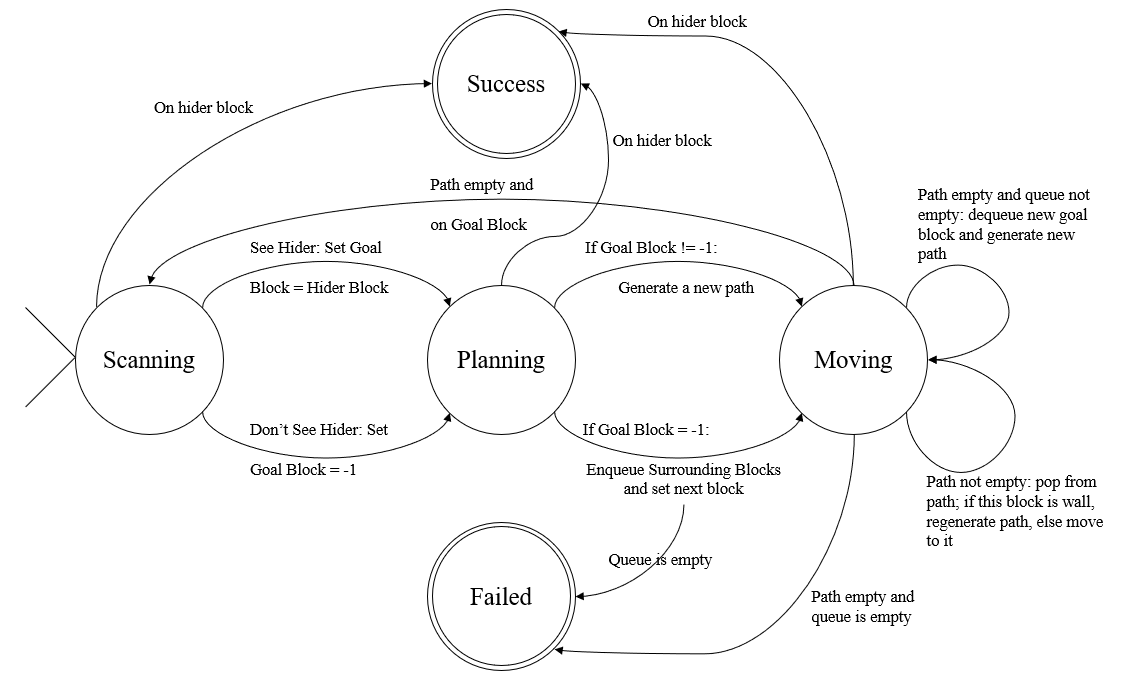
\includegraphics[width=1\linewidth]{bfsfa.PNG} 
\caption{A deterministic finite automaton representing the Modified Breadth-First Search Algorithm.}
\end{figure} 

\subsubsection{Modified Depth-First Search}
Depth-First Search works in the a similar manner as Breadth-First Search but instead replaces the queue with a stack to store the nodes it has not yet visited. Using the stack, a Last-In-First-Out (LIFO, as compared to the queue's first-in-first-out, FIFO, system) motivates it to explore blocks farther from its position before exploring alternative paths close to it\footnote{Theoretically, with the addition of the Scanning mode or state, this algorithm should discover the hider quicker on average, especially in maps where the hider is far away from the seeker, because the seeker is motivated to explore deep paths fist. However, we shall see if this theory is borne out in the experimental results.}. This seeker uses the exact same strategy as the one in \textbf{Section \ref{BFS}}, internally using a stack and pushing and popping to and from that data structure.

\subsubsection{Randomization}
Instead of having each of these Graph-Based models explore its neighboring blocks in a deterministic fashion (i.e. South, then South-East, then East, etc.), which could potentially bias certain maps which have the hider in a certain direction from the start, I have chosen to randomize the order. Running multiple experiments, as outlined in \textbf{Section \ref{Experiments}}, allows this randomization to even out into a mean time for a particular map.

\subsubsection{Graph-Based Models: Future Improvements}
A future improvement to these models could be utilizing the scanning mode to more quickly prune the graph of wall blocks. When the seeker casts out eight rays, some of these hit inner walls, which it can then remove from the graph. This would eliminate wasted time using these blocks in paths or examining them as potential blocks for the queue or stack. Especially in the case of breadth-first search, this means the seeker would not have to travel back across the map just to discover that all the potential edges of its new block lead to walls.

\subsection{Corner- and Room-Based Model}

\subsubsection{Overview}
The Corner- and Room-Based Model\footnote{Note that a consequence of the structure of $ BG $ is that the seeker can slip through cracks in corners (i.e. if we have a $ 2 \times 2 $ grid where the northwest block and the southeast block are walls and the others are not, the graph-based seeker can still get through, but the Corner- and Room-Based Model may not be able to). This should be standardized in future versions, whether by allowing the Corner- and Room-Based seeker to perform similar jumps or catching these jumps in the graph-based models.} is another seeking algorithm which, instead of exploring the graph $ BG $ alone, explores $ BG $ and $ EG $, thus investigating the hider's position by inspecting the structure of the environment itself. Unlike the Graph-Based models, this model internally stores both an edge graph and a block graph. 

This model attempts to model human-like behavior. In contrast to the Graph-Based models, this model can see in one line at a time\footnote{Future improvements could make use of some sort of ``vision cone'' to approximate human sight.}.

This model also works like a deterministic finite automaton, transitioning to different states based on the information it discovers in each iteration. The following subsections will explore these various states. As with the Graph-Based models, at every step the seeker checks to see if it is on the block of the hider; if so, it transitions to the success state.

\subsubsection{Scan}

The model starts in this state. A full scan consists of looking in each of the eight directions, but each step is made up of a single direction. Thus, internally, the seeker stores how much it has currently rotated during its Scan phase, transitioning to the next state based on what it sees during its full Scan.

Each Scan casts a ray in the direction in which the seeker is currently looking. If this ray hits the hider, it takes a step in the hider's direction. Otherwise, we can mark some number of edges\footnote{Internally, edges in $ EG $ are represented as being in one of several states: InnerWall, OuterWall, Seen, or Unknown. All edges in $ EG $ start in the Unknown state and then are marked as one of the other states as the seeker explores its environment.}\textsuperscript{,}\footnote{Getting the edges on a path when the direction is wholly horizontal or vertical is a trivial matter. In this case, just take the end point of the path (i.e. the hit point of the ray) and subtract or add to the $ x $ or $ y $ component by the size of a block (we have used one as this size) until reaching the seeker's position. Getting the edges on a diagonal path of a potentially arbitrary angle is more complex. For this, define $ (x_{hit}, y_{hit}) $ and $ (x_{seeker}, y_{seeker}) $ as the coordinates of the ray's hit and the seeker, respectively. Then, the slope of the line segment connecting these two points is given by $ m = \frac{y_{hit}-y_{seeker}}{x_{hit}-x_{seeker}} $ and the intercept (if the line segment was drawn out to a full line) is given by $ b = y_{i} - m \cdot x_{i} $ where $ (x_{i}, y_{i}) $ can be either the hit point or the seeker's point. Then the set of points on the path are given by all the points on this line segment, that is, the points $ (x, y) $ on $ y = m \cdot x + b $ where $ \min(x_{hit},x_{seeker}) \leq x \leq \max(x_{hit}, x_{seeker}) $ and $ \min(y_{hit},y_{seeker}) \leq y \leq \max(y_{hit},y_{seeker}) $ where $ (x, y) $ are on an edge of the graph. In our graph this is a matter of whether the $ x $ or $ y $ component is an integer.}. If the last of these points is not on the outer wall of our map\footnote{Note that this definition relies on where the origin in the coordinate space lies on the graph (i.e. which node it falls on in $ EG $). If we let this origin point be $ (x_{origin}, y_{origin}) $ where both components are positive if the origin falls within the graph (e.g. if the origin point falls on row 8 and column 4, counting the point on 0-th row and 0-th column as the upper left corner of the map, it is represented as $ (4, 8) $, then we define the in-bounds x coordinates as $ -x_{origin} < x < cols - x_{origin} $ and the in-bounds y coordinates as $ y_{origin} - rows < y < y_{origin} $. Points of equality define the outer walls of the map.}, we know that the edge on which that point lies is an inner wall. If we have not yet seen the wall on which this point lies\footnote{Internally, the seeker stores a list of walls where walls are bounded by points $ (x_{1}, y_{1}) $ and $ (x_{2}, y_{2}) $ and either $ \left|x_{2}-x_{1}\right| = 0 $ or $ \left|y_{2}-y_{1}\right| = 0 $. There are, therefore, no diagonal walls.}, we add this point to an internal list to examine in the next state. Otherwise each edge that is not the last (since the last edge is either an inner wall or an outer wall) is marked as Seen\footnote{If the direction of the ray is exactly $ 45^{\circ} $,  $ 135^{\circ} $, $ 225^{\circ} $, or $ 315^{\circ} $, then the ray runs through only nodes. In this case, for pairs of nodes which are not the last pair, we mark all the edges of the block bounded by the pair of nodes as seen. Let the pair of nodes be represented by $ n_{0} $ and $ n_{1} $, where $ n_{1} $ is the greater of the two. If $ n_{1} - n_{0} = cols + 2 $, then these edges, if they are in bounds, are given by $ (n_{0}, n_{0} + cols + 1) $, $ (n_{0}, n_{0} + 1) $, $ (n_{1} - (cols + 1), n_{1}) $, and $ (n_{1} - 1, n_{1}) $. If $ n_{1} - n{0} = cols $, then these edges, if they are in bounds, are given by $ (n_{0}, n_{0} + cols + 1) $, $ (n_{0} -1, n_{0}) $, $ (n_{1} - (cols + 1), n_{1}) $, and $ (n_{1}, n_{1} + 1) $. We know that we can do this because the ray crosses through the entire block unscathed and thus there is not a wall block in this position.}\textsuperscript{,}\footnote{We can map a point in the coordinate space to an edge in $ EG $ in the following manner. Let $ (x,y) $ be the coordinates of a point. If $ x $ and $ y $ are both integers, then we have a node given by $ (x + x_{origin}) \cdot (-y + y_{origin}) + (x + x_{origin}) + (-y + y_{origin}) $. Otherwise, if the $ x $ coordinate is an integer and the $ y $ coordinate is not, then we have an edge bounded by the following definition. Let $ row_{low} = \min(-\floor{y} + y_{origin}, -\ceil{y} + y_{origin}) $ and $ row_{high} = \max(-\floor{y} + y_{origin}, -\ceil{y} + y_{origin}) $. Let $ col = x + x_{origin} $. Then the edge is bounded by the nodes $ col \cdot row_{low} + col + row_{low} $ and $ col \cdot row_{high} + col + row_{high} $. If the $ y $ coordinate is an integer and the $ x $ coordinate is not, then we have an edge bounded by the following definition. Let $ row = -y + y_{origin} $. Let $ col_{low} = \min(\floor{x} + x_{origin}, \ceil{x} + x_{origin}) $ and $ col_{high} = \max(\floor{x} + x_{origin}, \ceil{x} + x_{origin}) $. Then the edge is bounded by the nodes $ col_{low} \cdot row + col_{low} + row $ and $ col_{high} \cdot row + col_{high} + row $}.

Once the scanner has completed a full $ 360^{\circ} $ scan, if it has wall points at which to look, it transitions to the ScanWall state. Otherwise, it transitions to the EnvironmentLearn state.

\subsubsection{ScanWall}

At the beginning of a run through this state, if there are no more wall points to look at, the seeker transitions to the EnvironmentLearn state. Otherwise, it pops a point off the list of wall points and faces it. If it has seen the wall on which this point lies already, it gets a new one (transitioning to the EnvironmentLearn state if the list is exhausted). The seeker then rotates to face this point and decides whether to scan the wall left or right first; this decision is based on which ray cast at a certain offset from this point is closer to the seeker and still on an inner wall. It then begins scanning the wall. 

On each step of scanning the wall, the seeker knows the ray cast hit point of its current direction and the previous hit point\footnote{On each update, it rotates by a certain amount, which was set at $ 1^{\circ} $ in the implemented algorithm.}. If the new hit point has departed from the currently scanned wall\footnote{Here we define this as if the new hit point lies on the outer boundary (see footnote 17 for the definition), if the distance between the two points is greater than a certain epsilon (chosen as $ 0.5 $) or, based on if the wall is horizontal or vertical, if the $ y $ or $ x $ coordinate, respectively, has started to change. Note that we can also halt early if we enter a previously seen wall.}, then we can use the most recent hit point as a potential corner. If we have not seen this corner before and this corner is not on a wall we have seen, we add it to a list of corners to which we may be able to move.

We then start to scan back in the opposite direction for our next corner point. Once we discover this corner, we define a new wall as the line segment bounded by these two corners\footnote{Note that this wall may potentially merge with existing walls. For example, if we have a wall from $ (0, 0) $ to $ (0, 3) $ and discover a new wall from $ (0, 3) $ to $ (0, 6) $, we can merge these into one wall stretching from $ (0, 0) $ to $ (0, 6) $.}. We then move to the next state (potentially staying in this one as expressed by the rules above). 

Note that at every step in the Scan and ScanWall state, when we see a wall, we remove the block beyond it from $ BG $.

\subsubsection{EnvironmentLearn}

This is a state specifically for coalescing information about the environment into informed decisions about where to move next. 

First, the seeker ensures that every edge on every wall it knows about is marked as an InnerWall. Then, it merges any walls which it has not already merged. It then attempts to make a room from its known walls\footnote{The seeker starts with knowledge of four walls: the top, right, bottom, and left boundaries of the map. These walls are referred to as ``permanent'' and can never be removed from this list. All other walls can be subsumed into rooms and removed from the list of walls accordingly (so as not to accidentally make the same room twice).}.

We define a \textbf{room} by the following definition: an area of space bounded by four walls, at most two of which are outer boundary walls, with one ``gap''\footnote{Let $ wall_{h_{0}} $ and $ wall_{h_{1}} $ be horizontal walls with a given $ y_{i} $ coordinate and $ x_{i_{min}} $ and $ x_{i_{max}} $ bounds ($ i \in \{0, 1\} $). Let $ wall_{v_{0}} $ and $ wall_{v_{1}} $ be vertical walls with a given $ x_{k} $ coordinate and $ y_{k_{min}} $ and $ y_{k_{max}} $ bounds ($ k \in \{0, 1\} $). A horizontal wall is separated from the vertical walls if the following: $ \neg (x_{i_{min}} \leq \min(x_{0}, x_{1}) \wedge  x_{i_{max}} \geq \max(x_{0}, x_{1})) $. A vertical wall is separated from the horizontal walls if the following: $ \neg (y_{i_{min}} \leq \min(y_{0}, y_{1}) \wedge y_{i_{max}} \geq \max(y_{0}, y_{1})) $.}. The restriction to one ``gap'' is included to restrict corridors or hallways from being included as rooms, but this may prevent larger maps where rooms with multiple entries and exits from being properly explored. An example map, shown in \textbf{Figure 2}, helps demonstrate why portions of this definition were chosen\footnote{If the four walls pass the one ``gap'' test, for practicality we need to also ensure that the walls are not misaligned. Let $ x_{min} $ be the minimum of the $ x $ coordinates of the vertical walls (conversely, $ x_{max} $). Let $ y_{min} $ and $ y_{max} $ be defined similarly. A horizontal wall is misaligned if its maximum $ x $ coordinate is less than or equal to $ x_{min} $ or if its minimum $ x $ coordinate is greater than or equal to $ x_{max} $. A vertical wall is misaligned if its maximum $ y $ coordinate is less than or equal to $ y_{min} $ or if its minimum $ y $ coordinate is greater than or equal to $ y_{max} $.}.

\begin{figure}[htbp]
\centering
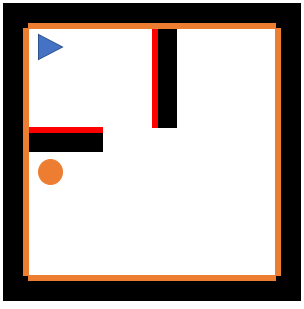
\includegraphics[width=0.5\linewidth]{mapex1.PNG} 
\caption{An example environment demonstrating the definition of a room.}
\end{figure} 

After an iteration through the Scan state, the seeker knows about the inner walls marked by the red lines. The outer boundary lines are marked in orange for illustrative purposes. 

\textbf{Figure 3} shows an example of why rooms are limited to at most two outer walls by highlighting a potential room which uses three outer walls in light yellow. 

\begin{figure}[htbp]
\centering
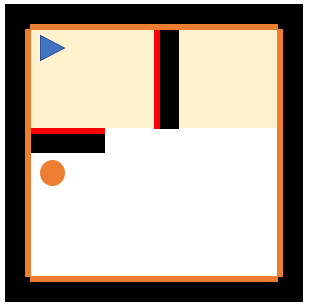
\includegraphics[width=0.5\linewidth]{wrongwalls.PNG} 
\caption{An example environment showing why we limit rooms to having at most two outer walls.}
\end{figure} 

The correct room is highlighted in green in \textbf{Figure 4}. However, another potential room is highlighted in light blue.

\begin{figure}[htbp]
\centering
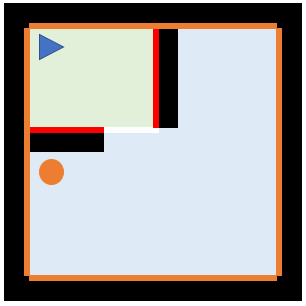
\includegraphics[width=0.5\linewidth]{potentialrooms.PNG} 
\caption{An example environment demonstrating potential rooms.}
\end{figure} 

Both potential rooms have one gap and at most two outer walls. Why, then, should we regard the green room as the only one we can know about? As a human observer, we can see that the blue room crosses over walls; further, we know that the seeker has only seen the blocks in the green area. It knows nothing about most of the blocks in the blue area and thus cannot say for sure about the status of this potential room. Because of this requirement, we test to see if all the blocks in our potential room are ``cleared,'' defined as every block in the room having no edges which are Unknown in $ EG $\footnote{We can map coordinates to blocks in the following fashion. We know that every point at which the seeker or hider can travel lies at the midpoint of a block. Since we have defined our blocks to have unit width and height, we can map the coordinates to a block as follows. Let $ (x, y) $ be the coordinates of a point. Let $ col = round (x + x_{origin} - 0.5) $ and $ row = round (-y + y_{origin} - 0.5) $. Then $ block = row \cdot cols + col $. We can reverse this mapping as follows. Let $ block $ be the block number of a given block. Then let $ row = block / cols $ and $ col = block \mod cols $. Then the coordinates of the midpoint of the block are $(-x_{origin} + col + 0.5, y_{origin} - row - 0.5) $.}\textsuperscript{,}\footnote{We then find the edges surrounding a block in the following way. We first find the coordinates of the block; let these be $ (x, y) $. Then the block's right edge is the edge mapped by $ (x + 0.5, y) $, the block's top edge is the edge mapped by $ (x, y + 0.5) $, the block's bottom edge is the edge mapped by $ (x, y - 0.5) $, and the block's left edge is the edge mapped by $ (x - 0.5, y) $. This mapping is covered in footnote 20.}. If the potential room is ``cleared,'' we identify a number of blocks which represent the room's entrance; these are blocks adjacent to the bound box of the room which do not hold wall blocks (i.e. they are not nodes we have removed from $ G $).  

If we successfully made a new room in this state, we know we have done all we can in this space, and therefore we need to leave it. To leave, we grab a random block from the room's entrance (setting it to the seeker's goal block), generate a path to it\footnote{This uses the same path-finding algorithm used in the Graph-Based models.}, and transition to the Move state. 

If no new room was created, we transition to the FindCorner state.

In this iteration of the model the hider is static and each room should only be entered once. However, in future research with a moving hider, the seeker stores rooms (along with their entrances) so it knows to which point it can go to gather information about a wide swath of the environment. 

\subsubsection{FindCorner}

In the FindCorner state, if our goal block is not set to $ -1 $, we generate a path to it and transition to the Move state.

If our goal block is $ -1 $, we examine potential corners. If there are no potential corners for us to explore (we have already explored every corner we've seen or the corner has been added to a room already), we transition to the Move state. Otherwise, we pop a corner off this list and examine it. The coordinate of the corner maps to a node in $ EG $ given by the following. Let $ (x,y) $ be the coordinates of the corner. Then, standardizing that with our given origin, we have $ (x_{map}, y_{map}) = (x+x_{origin},-y+y_{origin}) $. Then our node is given by $ y_{map} \cdot (cols + 1) + x_{map} $. This node has four potential edges emanating from it\footnote{Refer to the rules governing edges in $ EG $.}. Based on the current status of these edges, which we shall refer to as top, right, left, and down, we want to find a block to which we can move to gain more information about the environment\footnote{The currently implemented rules are:

If only one of the edges is unknown, we add blocks as follows. If the left is an inner wall, we look at pairs of the others: if the top and right are seen, we can add the southeast block and mark down as an inner wall; if down and right are seen, we can add the northeast block and mark top as an inner wall; if down is seen and right is an inner wall, then we can add both northern blocks; if top is seen and right is an inner wall, then we can add both southern blocks. If the right is an inner wall, we look at pairs of the others: if top and left are seen, we can mark down as a wall and add the southwest block; if down and left are seen, we can mark top as an inner wall and add the northwest block; if down is seen and right is an inner wall, we can add both southern blocks; if top is seen and left is an inner wall we can add both northern blocks.  We follow a similar process for if down and top are inner walls.

If none of the edges is unknown, we add blocks as follows. If left and down are inner walls, we add the southeast and northwest blocks. If left and top are inner walls, we add the northeast and southwest blocks. If right and top are inner walls, we add the northwest and southeast blocks. If right and down are inner walls, we add the southwest and northeast blocks. 

If three edges are unknown, we find the unknown edge, travel along it and repeat this algorithm at that point.

If two edges are unknown, we add blocks as follows. If left and down are inner walls, we add the southwest block. If left and top are inner walls, we add the northwest block. If right and top are inner walls, we add the northeast block. If right and down are inner walls, we add the southeast block. If left is an inner wall and down is seen, we add the southwest block. If right is an inner wall and down is seen, we add the southeast block. If left is an inner wall and top is seen, we add the northwest block. If right is an inner wall and top is seen, we add the northeast block. If top is an inner wall and right is seen, we add the northeastern block. If top is an inner wall and left is seen, we add the northwest block. If down is an inner wall and right is seen, we add the southeast block. Finally, if down is an inner wall and left is seen, we add the southwest block.}. We then pick a random block from among these options, set the goal block to it, generate a path, and transition to the Move state\footnote{As a ``cheat,'' if no blocks are found (i.e. we did not implement enough rules or implement them properly), we transition to the Move state anyways instead of failing. That state successfully handles moving to a location even if it does not have a goal block.}. 

\subsubsection{Move}
In the move state, the seeker first examines its path. If it has no blocks in its path to move, it finds a new place to go. First, it examines its potential eight surrounding blocks, identifying if it has not visited any of them. If such a block exists, it moves to it and transitions to the Scan state. Second, if no such block exists, the seeker finds a random block in the map it has not yet visited. If there is a path it can generate to this block, it uses this path (i.e. stays in this mode). If not, it keeps trying to find a block to which it can move until it can no longer do so. If it cannot find a block to which it can move, it moves to a Failed state.   

If the path does have a next block, it rotates to face this block and attempts to move. If it cannot move to this next location (i.e. the location is outside or it is inside a wall that has not been removed for some reason), it removes that block from the graph and generates a new path to the goal block. Note that we know that if there is no such path, the Move state will then attempt to try its random movement process. 

If the Move state successfully lands on the goal block, it transitions to the Scan state and resets the goal block to $ -1 $.

Note that at every step in the movement process, the seeker is looking in its direction for the hider and marking edges in $ EG $.

\subsubsection{Improvement}
As a slight improvement to reduce the gap between the Graph-based models and this model, a (``cheat'') step was added to every update where the seeker always looks in all eight directions for the hider, moving towards it if it sees it. 

\section{Experimental Setup} \label{Experiments}
In order to compare across models, we must set up a common testing environment and perform multiple runs of each, then average out their ability. Timing may not be the best metric of performance (for example, one of the goals of the Corner- and Room-based Model is to better approximate human-like behavior), but it can serve as an acceptable proxy. By running each of these models on differently structured maps multiple times, we can average across runs on a particular model to approximate their run-time. We can also collect data about each map including its sparsity (measured by numbers of wall blocks) and the distance between the hider and the seeker at the start to get a better sense of how each model performs under various conditions.

\subsection{Map Generation}
A solid experiment does its best to remove bias in its testing. Differently laid out maps may hold bias towards a particular model, so drawing models by hand may unintentionally aggravate those biases. Thus, we must come up with some algorithm for generating maps on which to experiment. 

A first, naive algorithm is to pick some random number of blocks out of the pool of available spaces and turn these into walls. Then place the hider and seeker randomly among the available remaining spaces. When using uniform probabilities over the total number of blocks (i.e. let the number of blocks be a random variable $ B $ where $ B = U(1, rows \cdot cols - 3 $ (where the $ - 3 $ is the usual $ - 1 $ plus 2 spaces for the hider and  seeker), this algorithm has an increased tendency to produce unsolvable maps where the hider and seeker are in their own holes of the map. Future work could alter this algorithm to use different probability distributions to produce different results (perhaps we can even design a probabilistic model such that walls are induced to be created, for example by weighting the neighboring blocks of a chosen wall block to have an increased probability of being walls as well.). This model has been implemented in the testing and is referred to as the \textbf{Random} algorithm.

A second algorithm uses the concept of walls to build a map with a more maze-like structure. This method is inspired by the Recursive Division algorithm for generating mazes, modified to produce more open spaces instead of tiny corridors\cite{Mazes}. The algorithm works as follows.

Let the parameters to the method be integers representing the bottom row, top row, left column, and right column (call these $ bottomRow $, $ topRow $, $ leftCol $, $ rightCol $). If $ leftCol \geq rightCol \lor bottomRow \geq topRow $, we exit. Then let $ width = rightCol - leftCol - 1 $ and $ height = topRow - bottomRow - 1 $. If either of these values are less than or equal to 1, we exit. Now let $ area = width \cdot height $. We define some value $ MAX\_AREA $\footnote{Chosen in the experiment to be 9.}; if $ area $ is less than this value, we exit. 

The Recursive Division algorithm for mazes swaps back and forth between writing horizontal and vertical walls, which inspires the creation of long, single width or height corridors. This algorithm instead picks randomly between the two options on every call. 

If horizontal is chosen, we pick a random row; that is, pick a random row $ r \in \{ bottomRow+1, \ldots, topRow - 1 \} $. Then pick a random amount of column values on that row; that is, pick some random number of values, from 0 to $ \left|C\right| $, from the set $ C = \{ leftCol+1, \ldots, rightCol - 1 \} $. Label all these values as walls. Now call this method recursively with parameters $ r $, $ topRow $, $ leftCol $, $ rightCol $ and $ bottomRow $, $ r $, $ leftCol $, $ rightCol $ (note that we use $ r $ instead of $ r + 1 $ or $ r - 1 $ because the algorithm excludes the values on the margins of the range). 

If vertical is chosen, we perform a similar procedure; pick a random column $ c \in \{ leftCol + 1, \ldots, rightCol - 1 \} $. Then pick a random amount of row values on that column; that is, pick some random number of values, from 0 to $ \left|C\right| $, from the set $ C = \{ bottomRow + 1, \ldots, topRow - 1 \} $. Label all the values as walls. Now call this method recursively with parameters $ bottomRow $, $ topRow $, $ c $, and $ rightCol $ and $ bottomRow $, $ topRow $, $ leftCol $, and $ c $. 

To start this algorithm, call it with the values $ -1 $, $ rows $, $ -1 $, $ cols $.

This algorithm tends to produce maps which have some room-like qualities, but can also suffer from accidentally placing walls beside one another, thereby blocking the seeker's progression. This chance, however, does give us an opportunity to test each model's ability to catch and control failure. 

This algorithm is referred to as \textbf{Algorithm} in the code and in the testing.

\section{Experimental Results}
We ran 250 maps of each map generation process with 100 iterations of each seeker algorithm. Each experiment on a given map generation algorithm gave us 100 pieces of data about each seeker algorithm, including whether the seeker found the hider on a given run and how long it took (in milliseconds) to halt (either in the success or failed state). In order to standardize the results, we disqualified any experiments which did not have all its runs result in the same value\footnote{To perform this, we took the number of successful runs for each of the DFS, BFS, and Corner- and Room-Based Models. If this number did not equal $ 0 $ - a successfully identified failed map - or $ 100 $ - a successfully identified successful map - we threw out the experiment from our data.}. This removal left us with $ 219 $ experiments through the Algorithm map generation process and $ 239 $ experiments through the Random map generation process.

The scarcities, measured by the total number of open blocks in the map\footnote{Remember that we have a $ 10 \times 10 $ map, so, for example, 77 wall blocks means a scarcity of $ 33 $.}, of the leftover runs are shown in the histogram in \textbf{Figure 5}.

\begin{figure}[htbp]
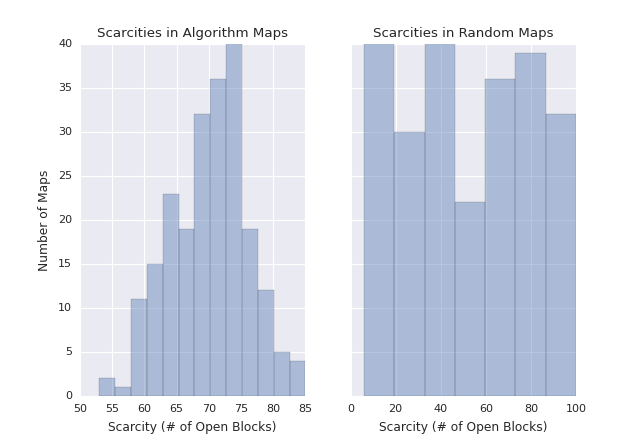
\includegraphics[width=1\linewidth]{Scarcity.png} 
\caption{Scarcities produced by each map generation algorithm.}
\end{figure} 

As expected, the Random algorithm produces a fairly uniform distribution of scarcities (given its uniform probabilities over number of wall blocks chosen). Interestingly, the Wall generation algorithm has a tendency to produce maps with a normal distribution of scarcity with a mean around $ 70 $ and a standard deviation around $ 6 $.

We have plotted all the results of each experiment as box plots in \textbf{Figure 6} through \textbf{Figure 15}. These show the mean time for each algorithm to halt along with whiskers indicating each algorithm's variability.

\begin{figure}[htbp]
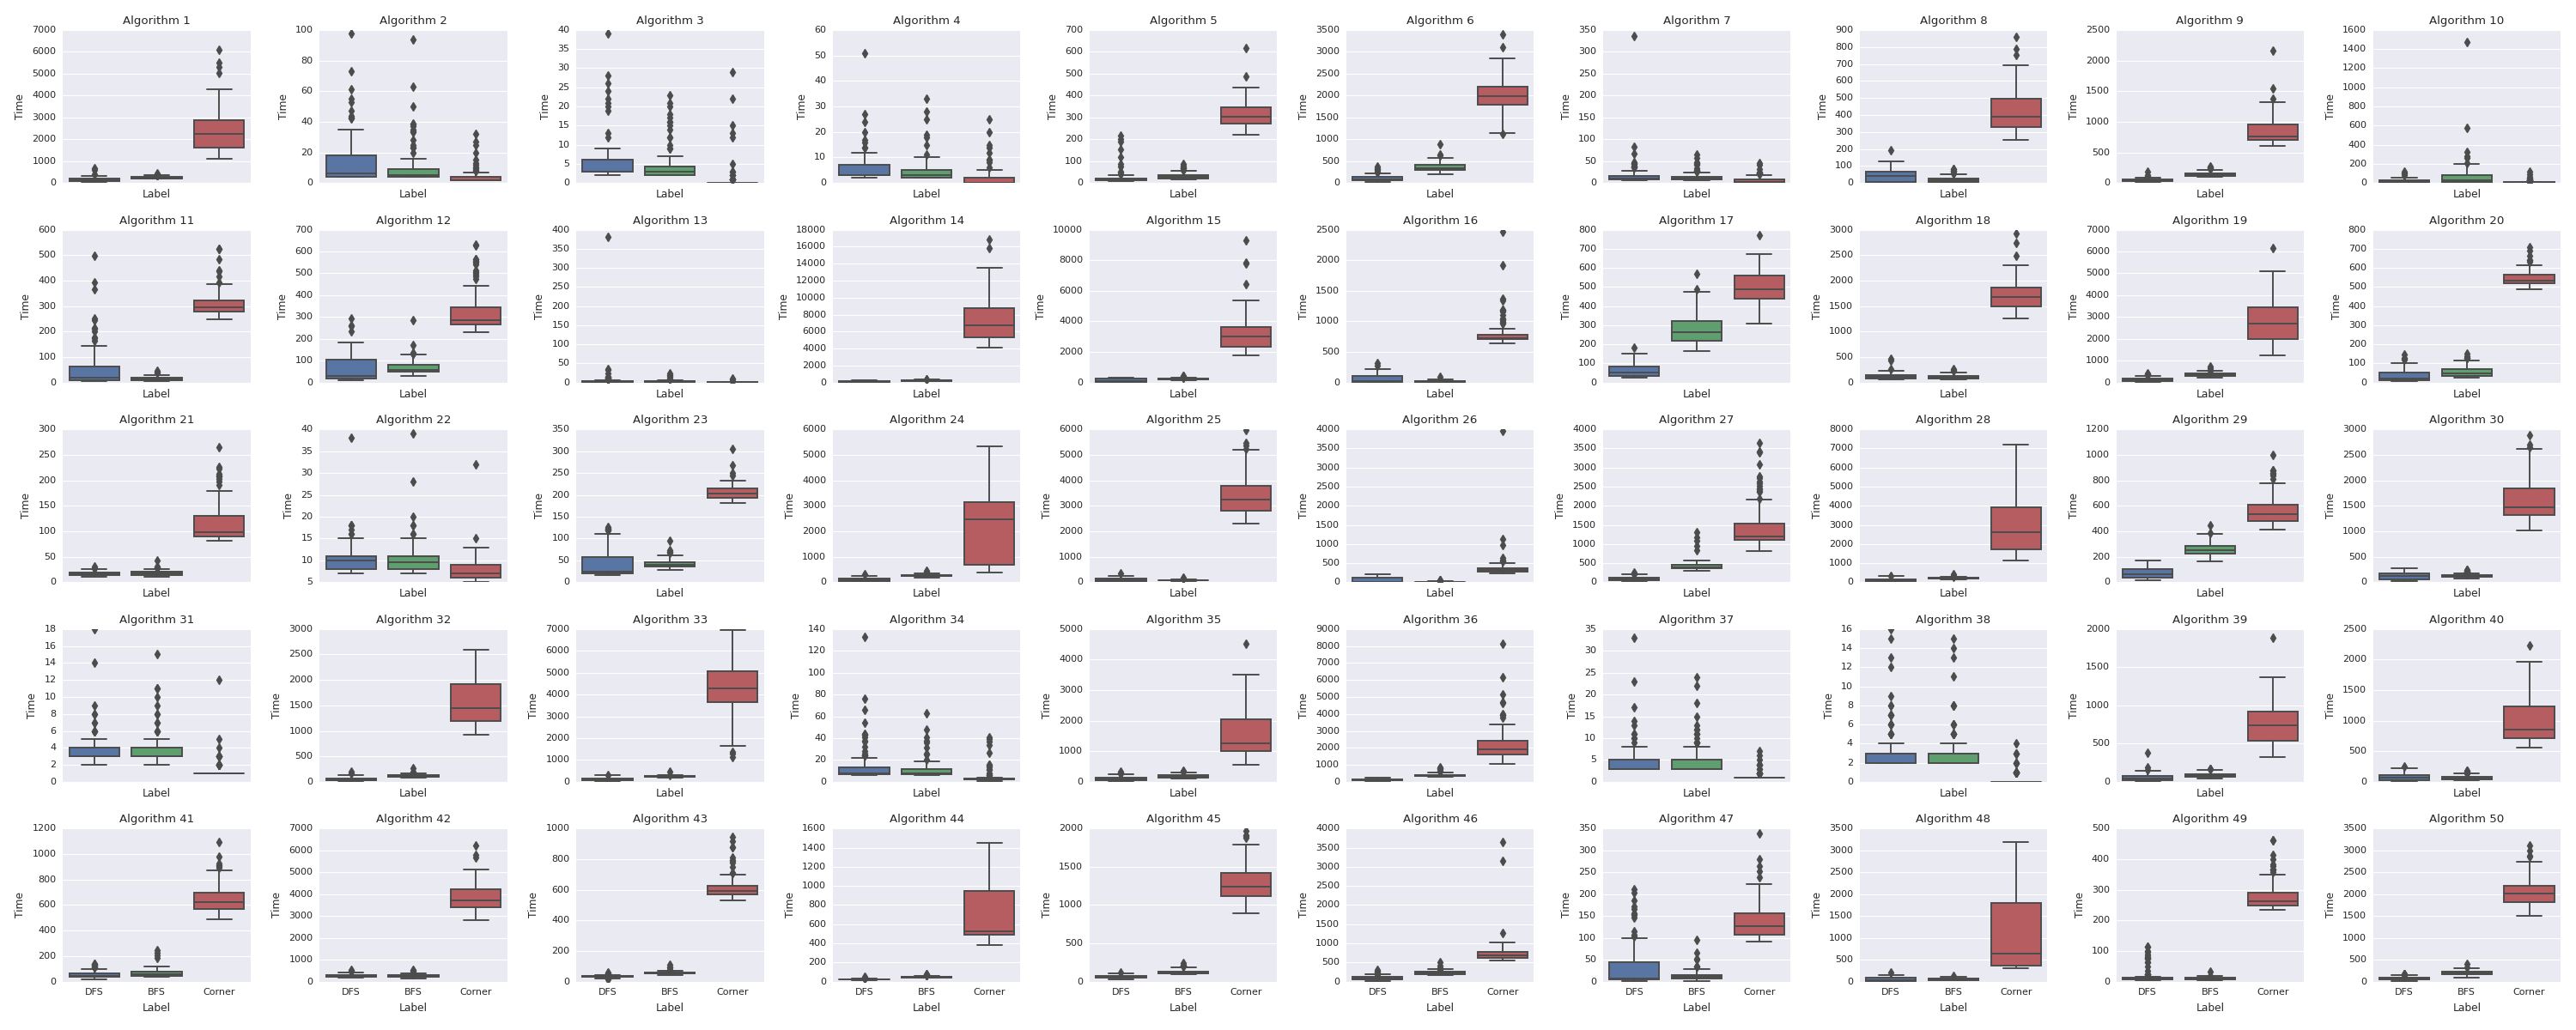
\includegraphics[width=1\linewidth]{Algorithm0-49.png} 
\caption{The results of Experiments 1-50 of the Algorithm experiments.}
\end{figure} 

\begin{figure}[htbp]
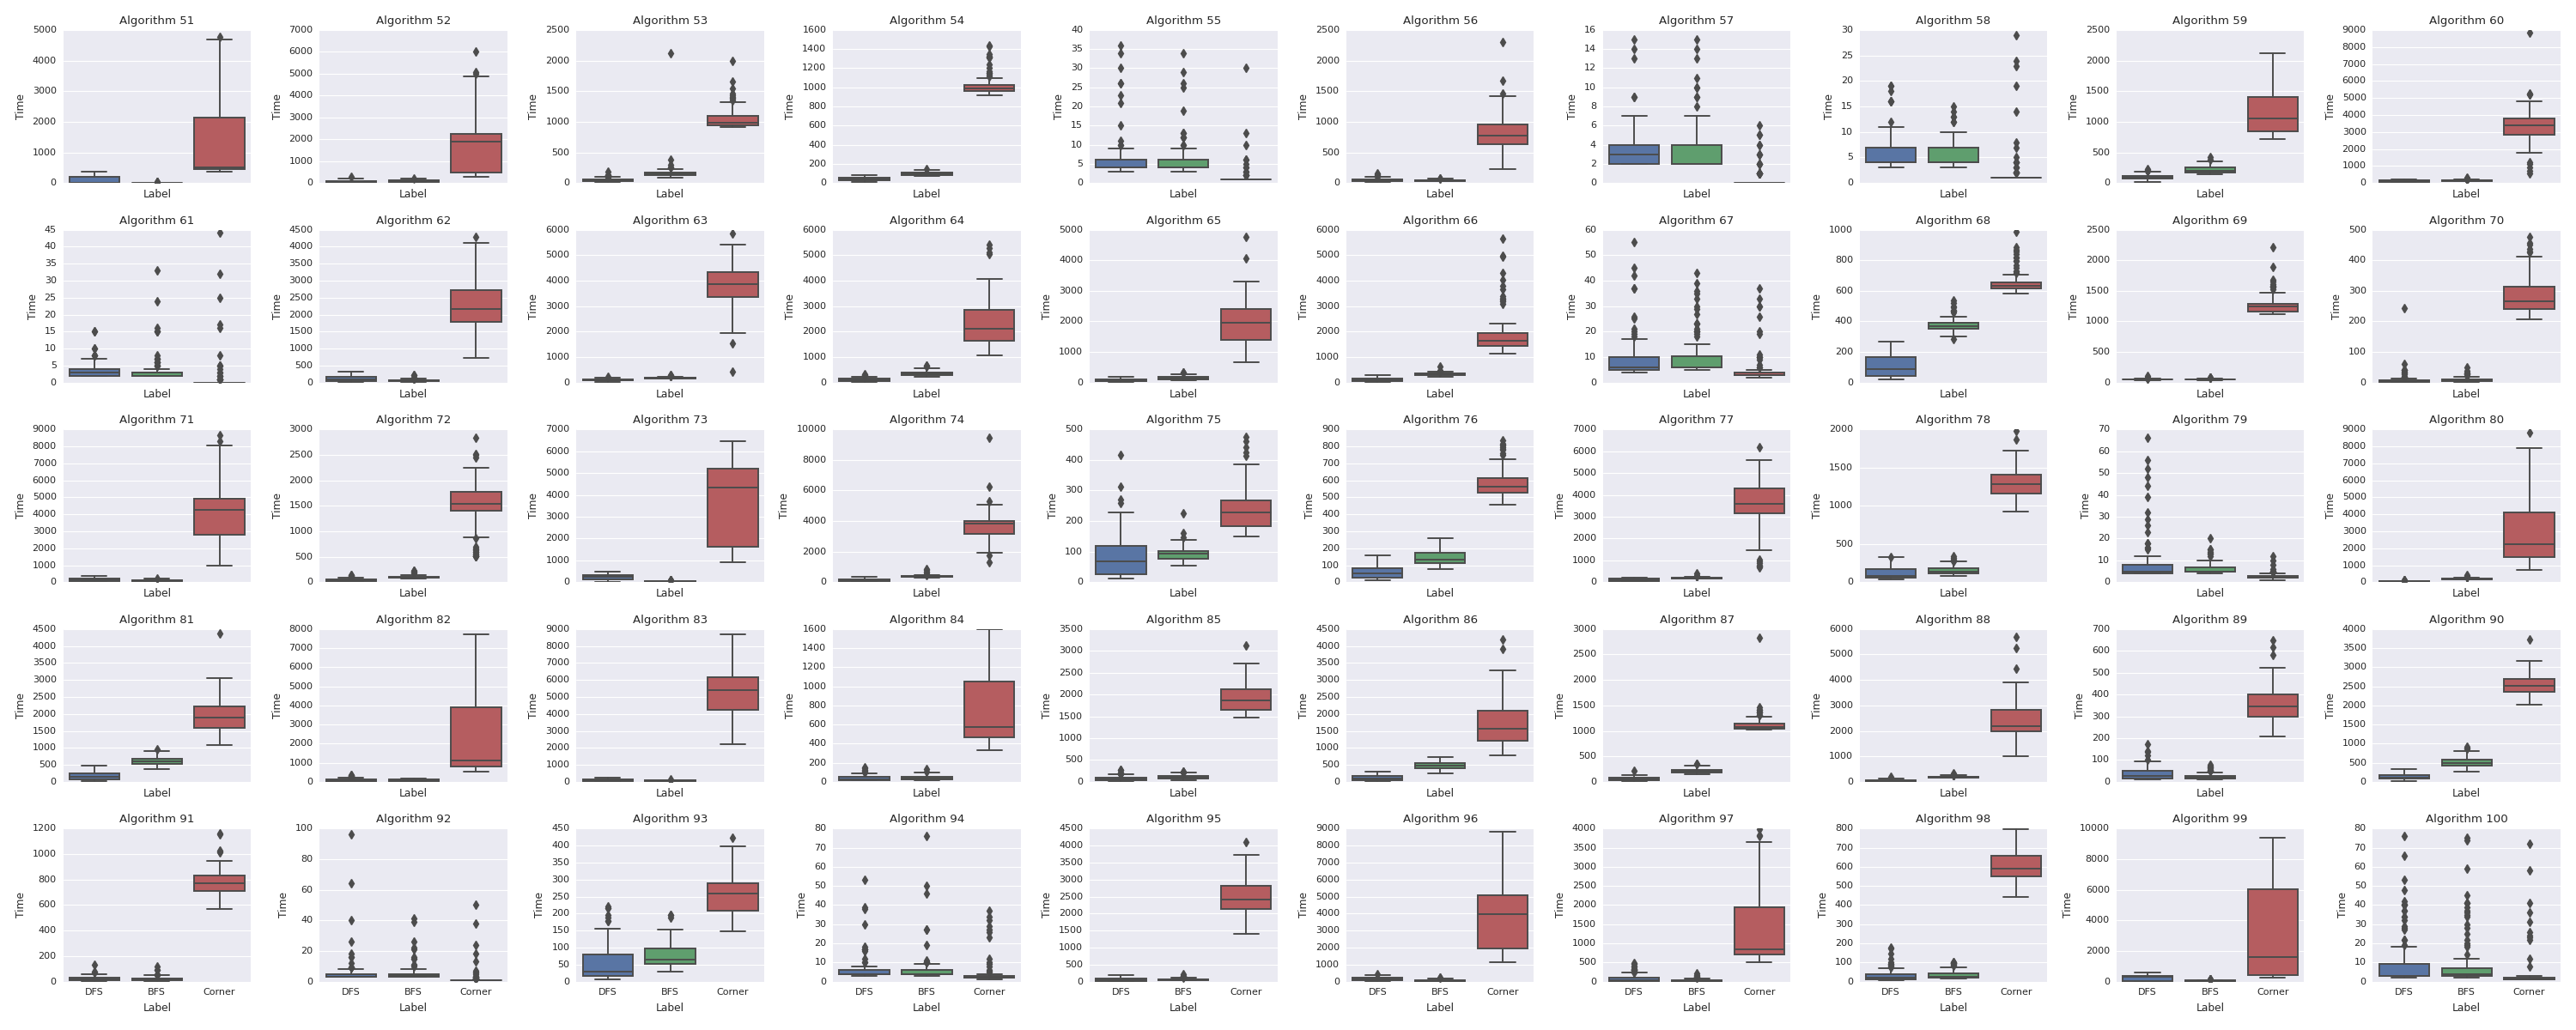
\includegraphics[width=1\linewidth]{Algorithm50-99.png} 
\caption{The results of Experiments 51-100 of the Algorithm experiments.}
\end{figure} 

\begin{figure}[htbp]
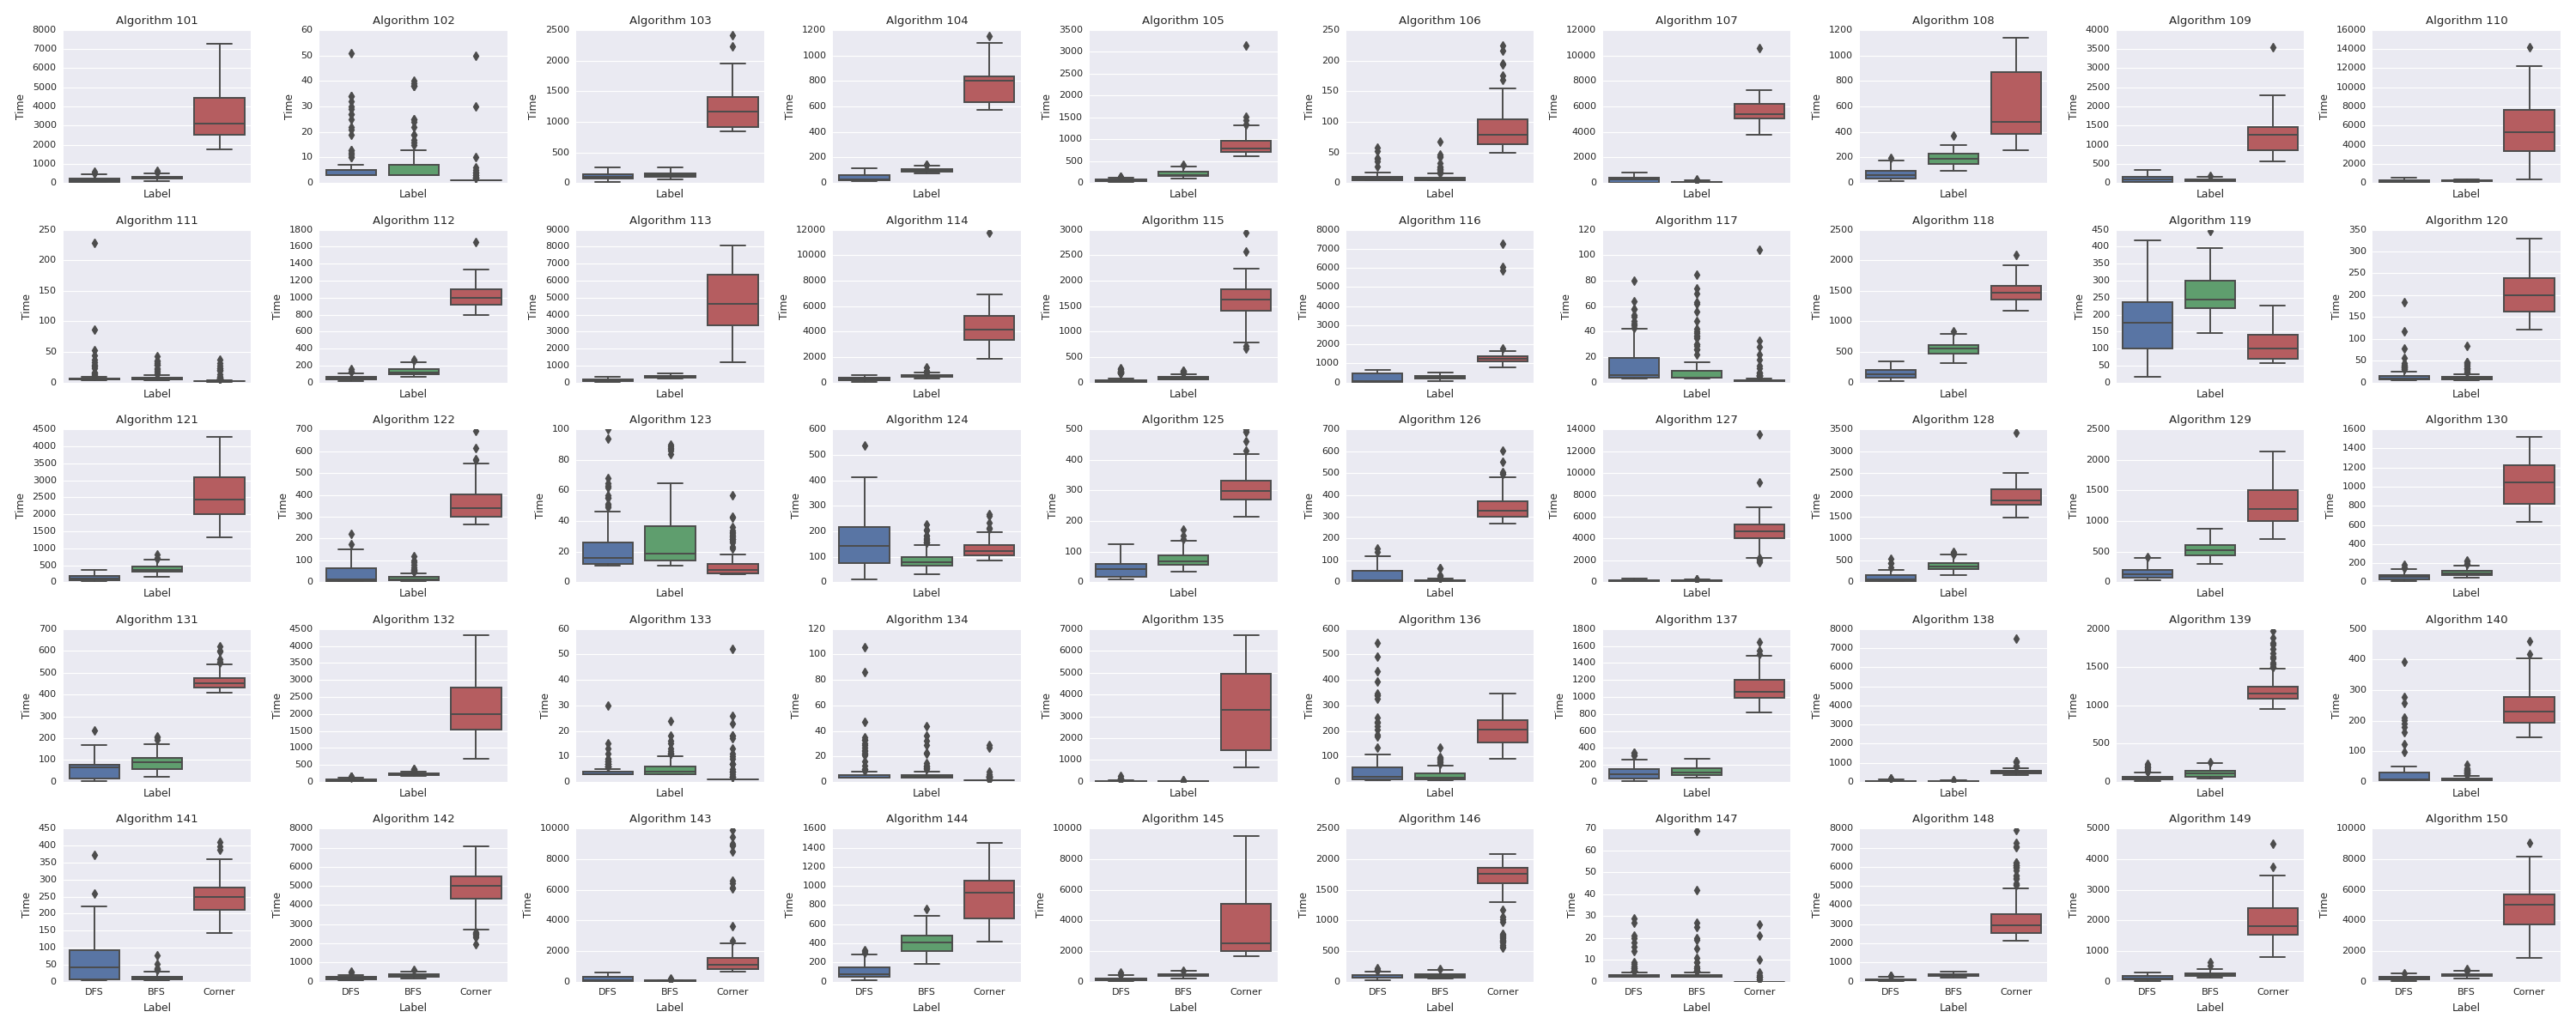
\includegraphics[width=1\linewidth]{Algorithm100-149.png} 
\caption{The results of Experiments 101-150 of the Algorithm experiments.}
\end{figure} 

\begin{figure}[htbp]
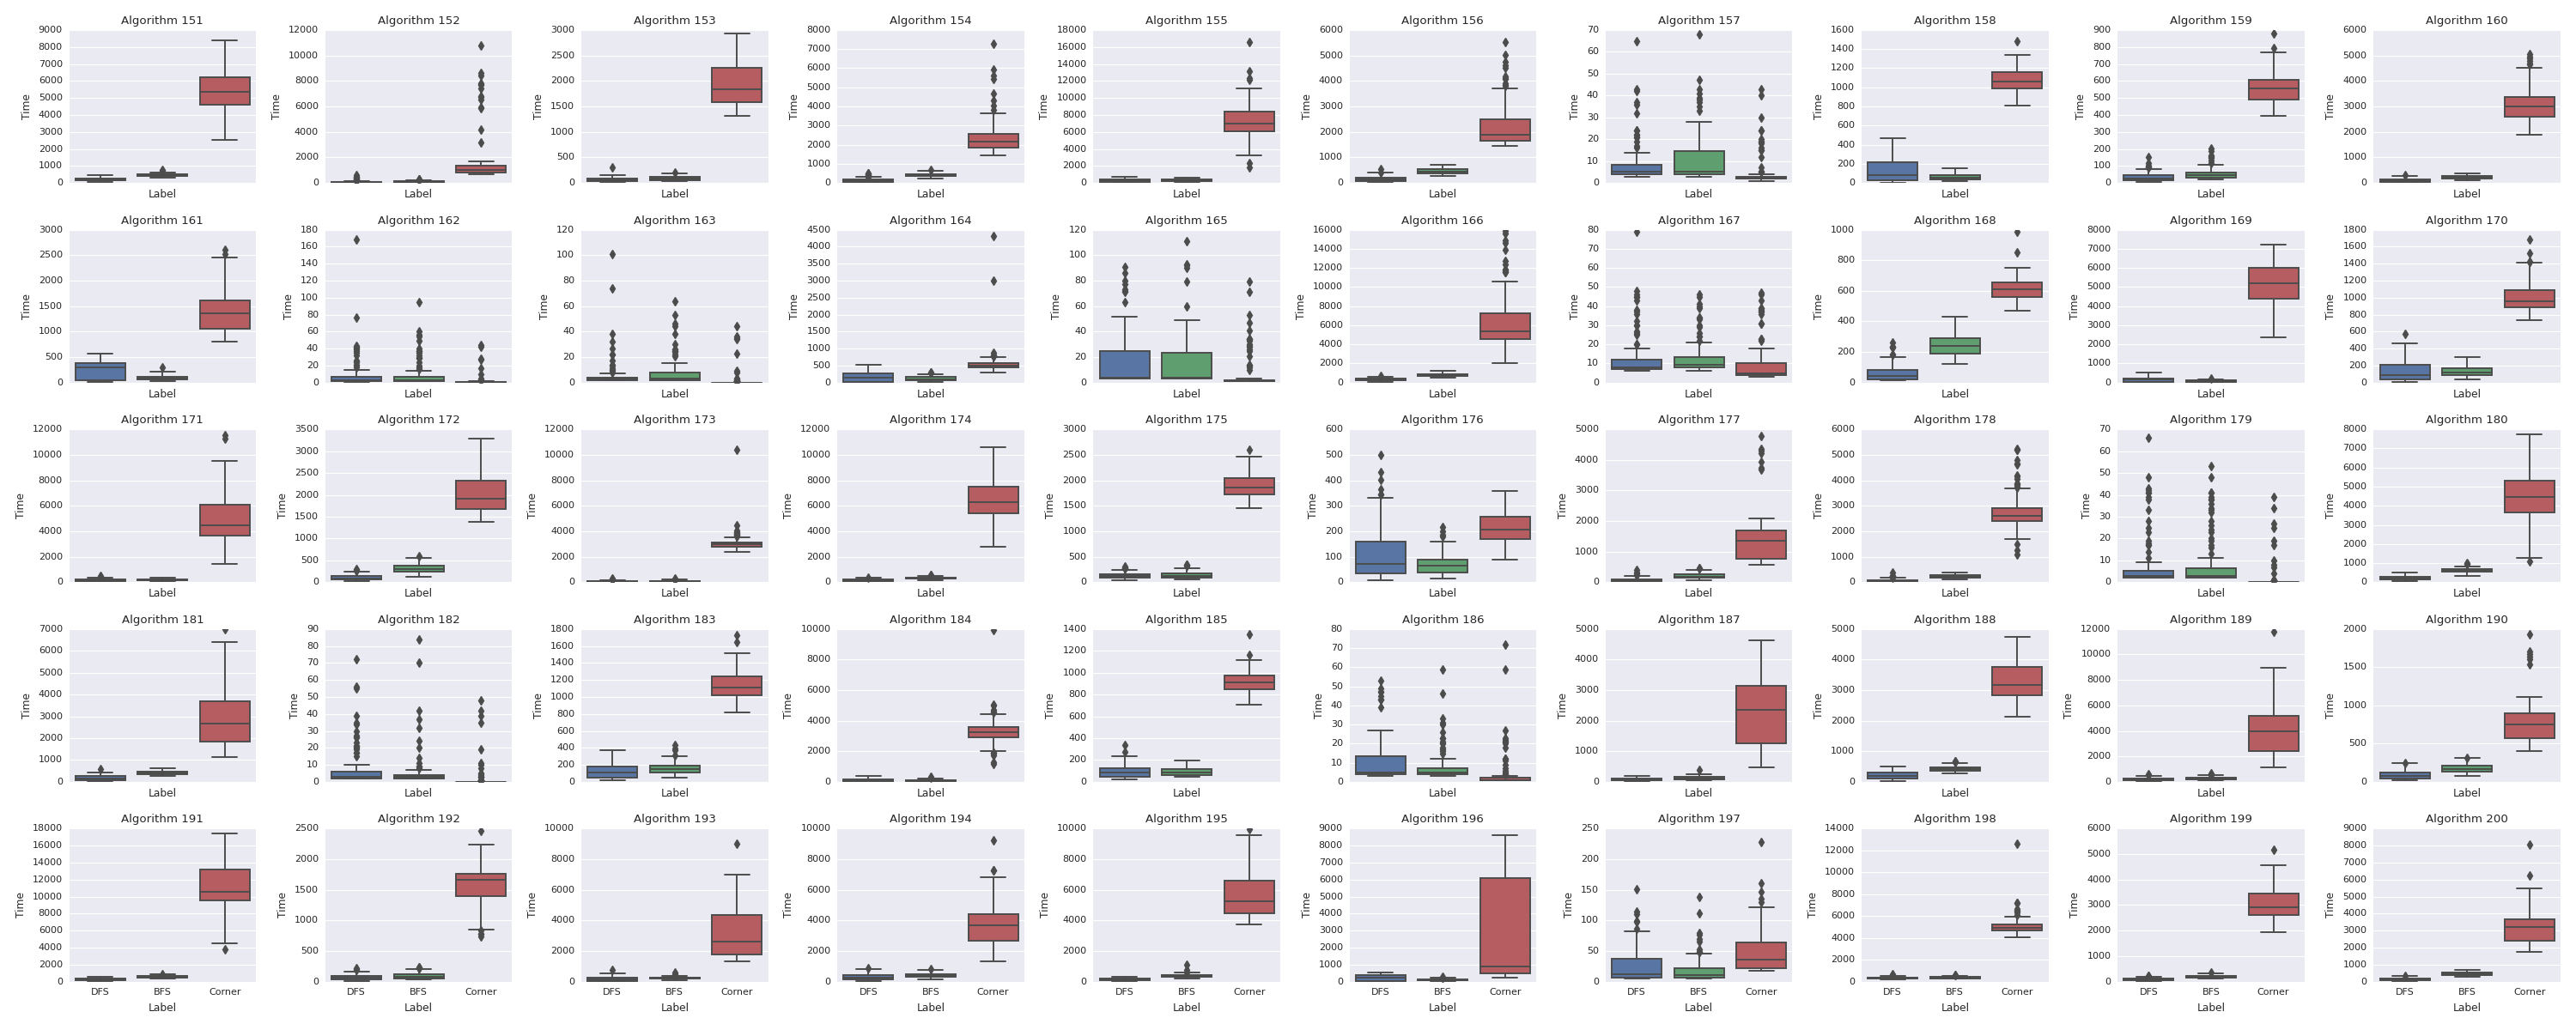
\includegraphics[width=1\linewidth]{Algorithm150-199.png} 
\caption{The results of Experiments 151-200 of the Algorithm experiments.}
\end{figure} 

\begin{figure}[htbp]
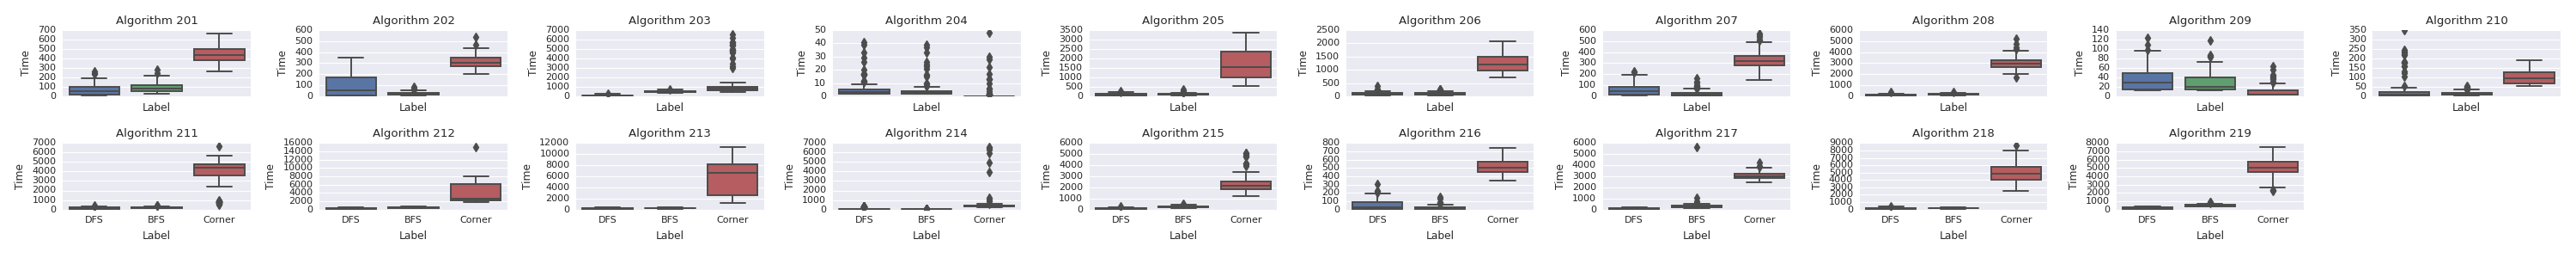
\includegraphics[width=1\linewidth]{Algorithm200-218.png} 
\caption{The results of Experiments 201-219 of the Algorithm experiments.}
\end{figure} 

\begin{figure}[htbp]
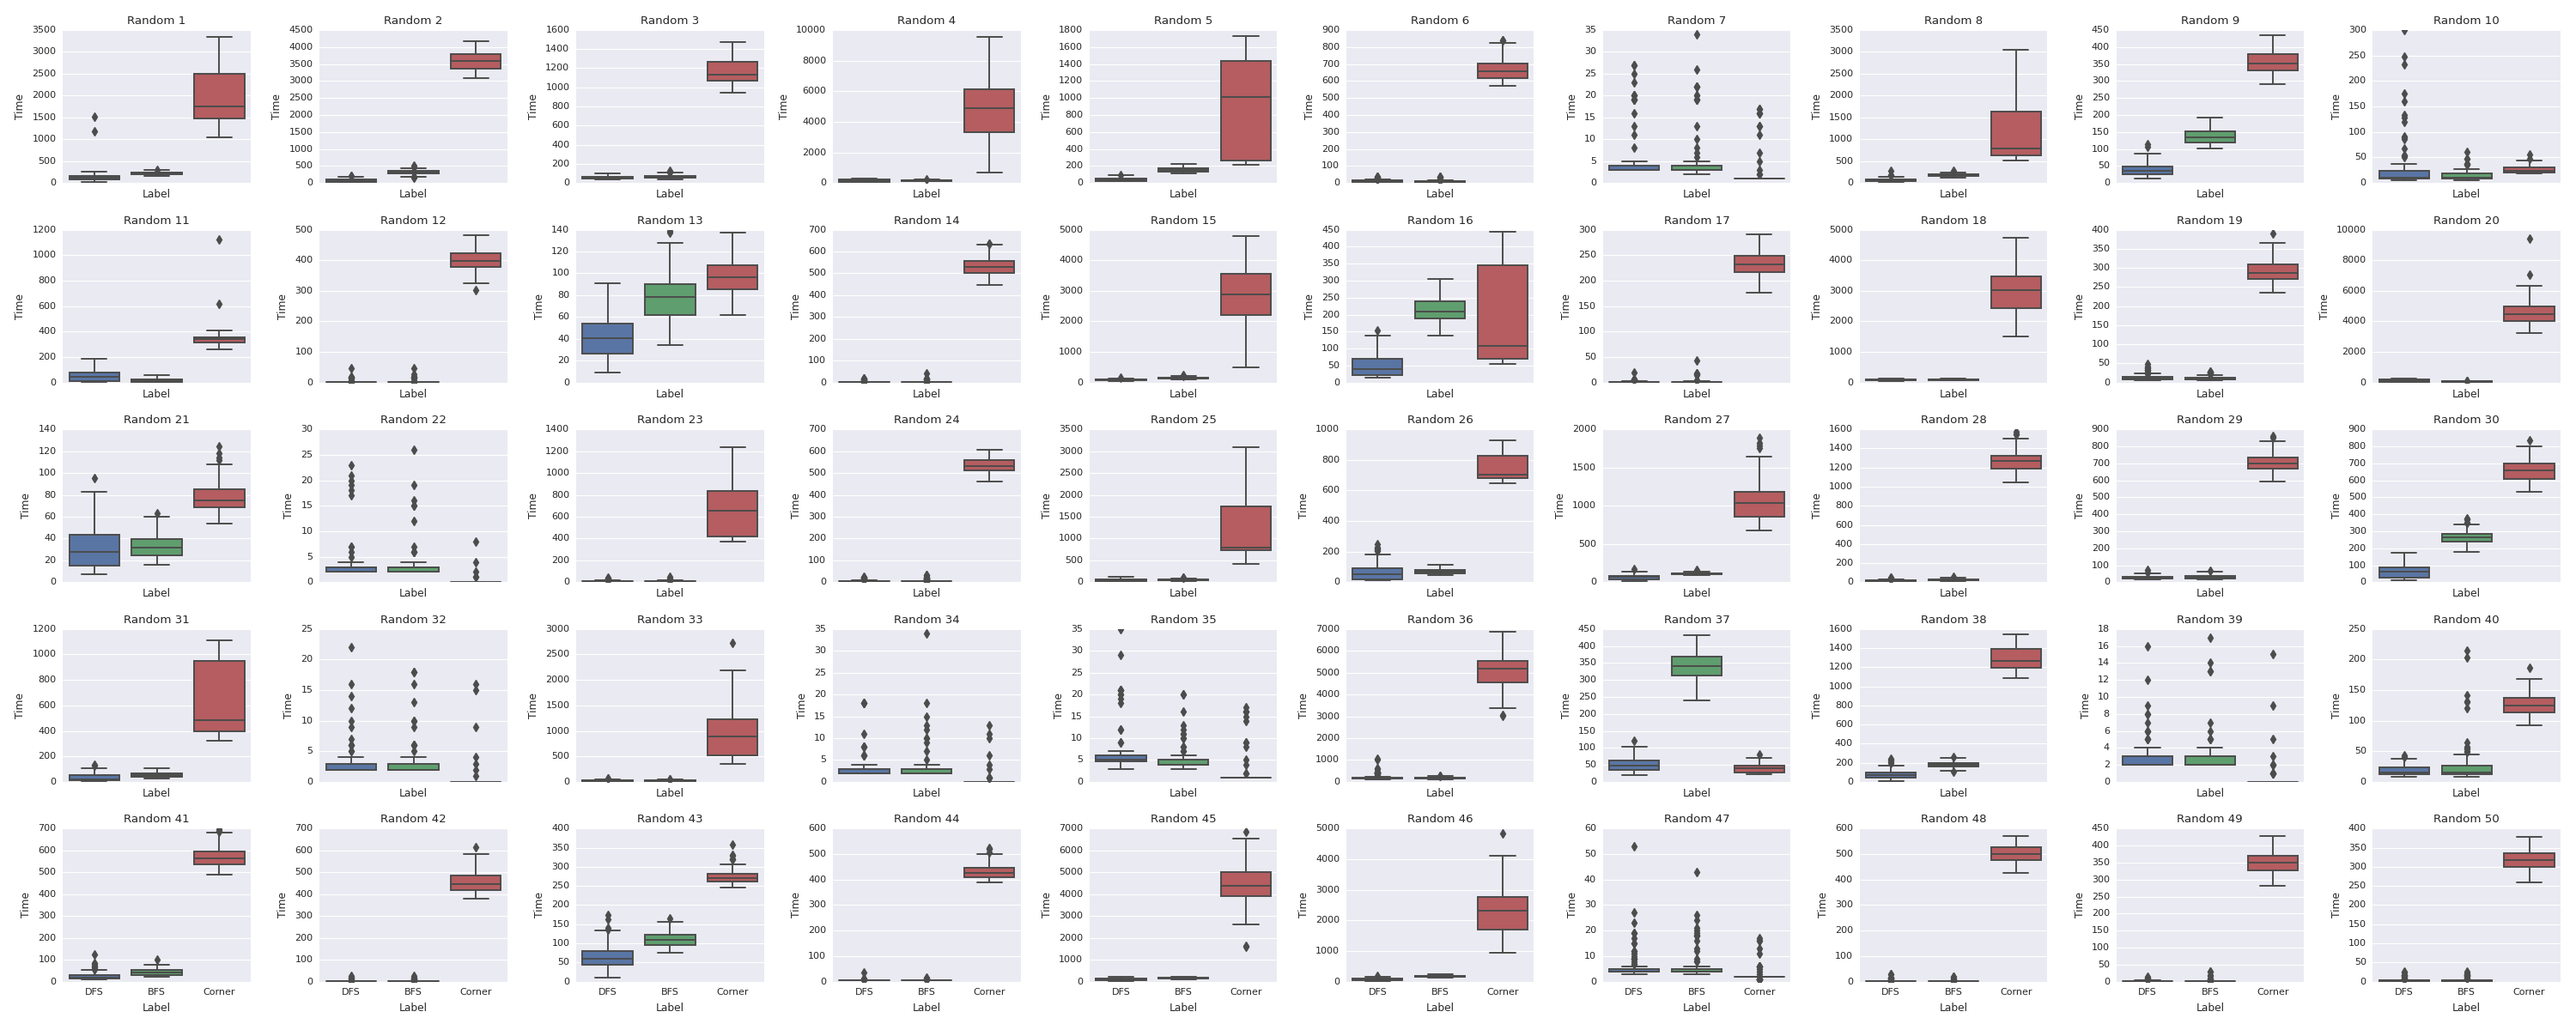
\includegraphics[width=1\linewidth]{Random0-49.png} 
\caption{The results of Experiments 1-50 of the Random experiments.}
\end{figure} 

\begin{figure}[htbp]
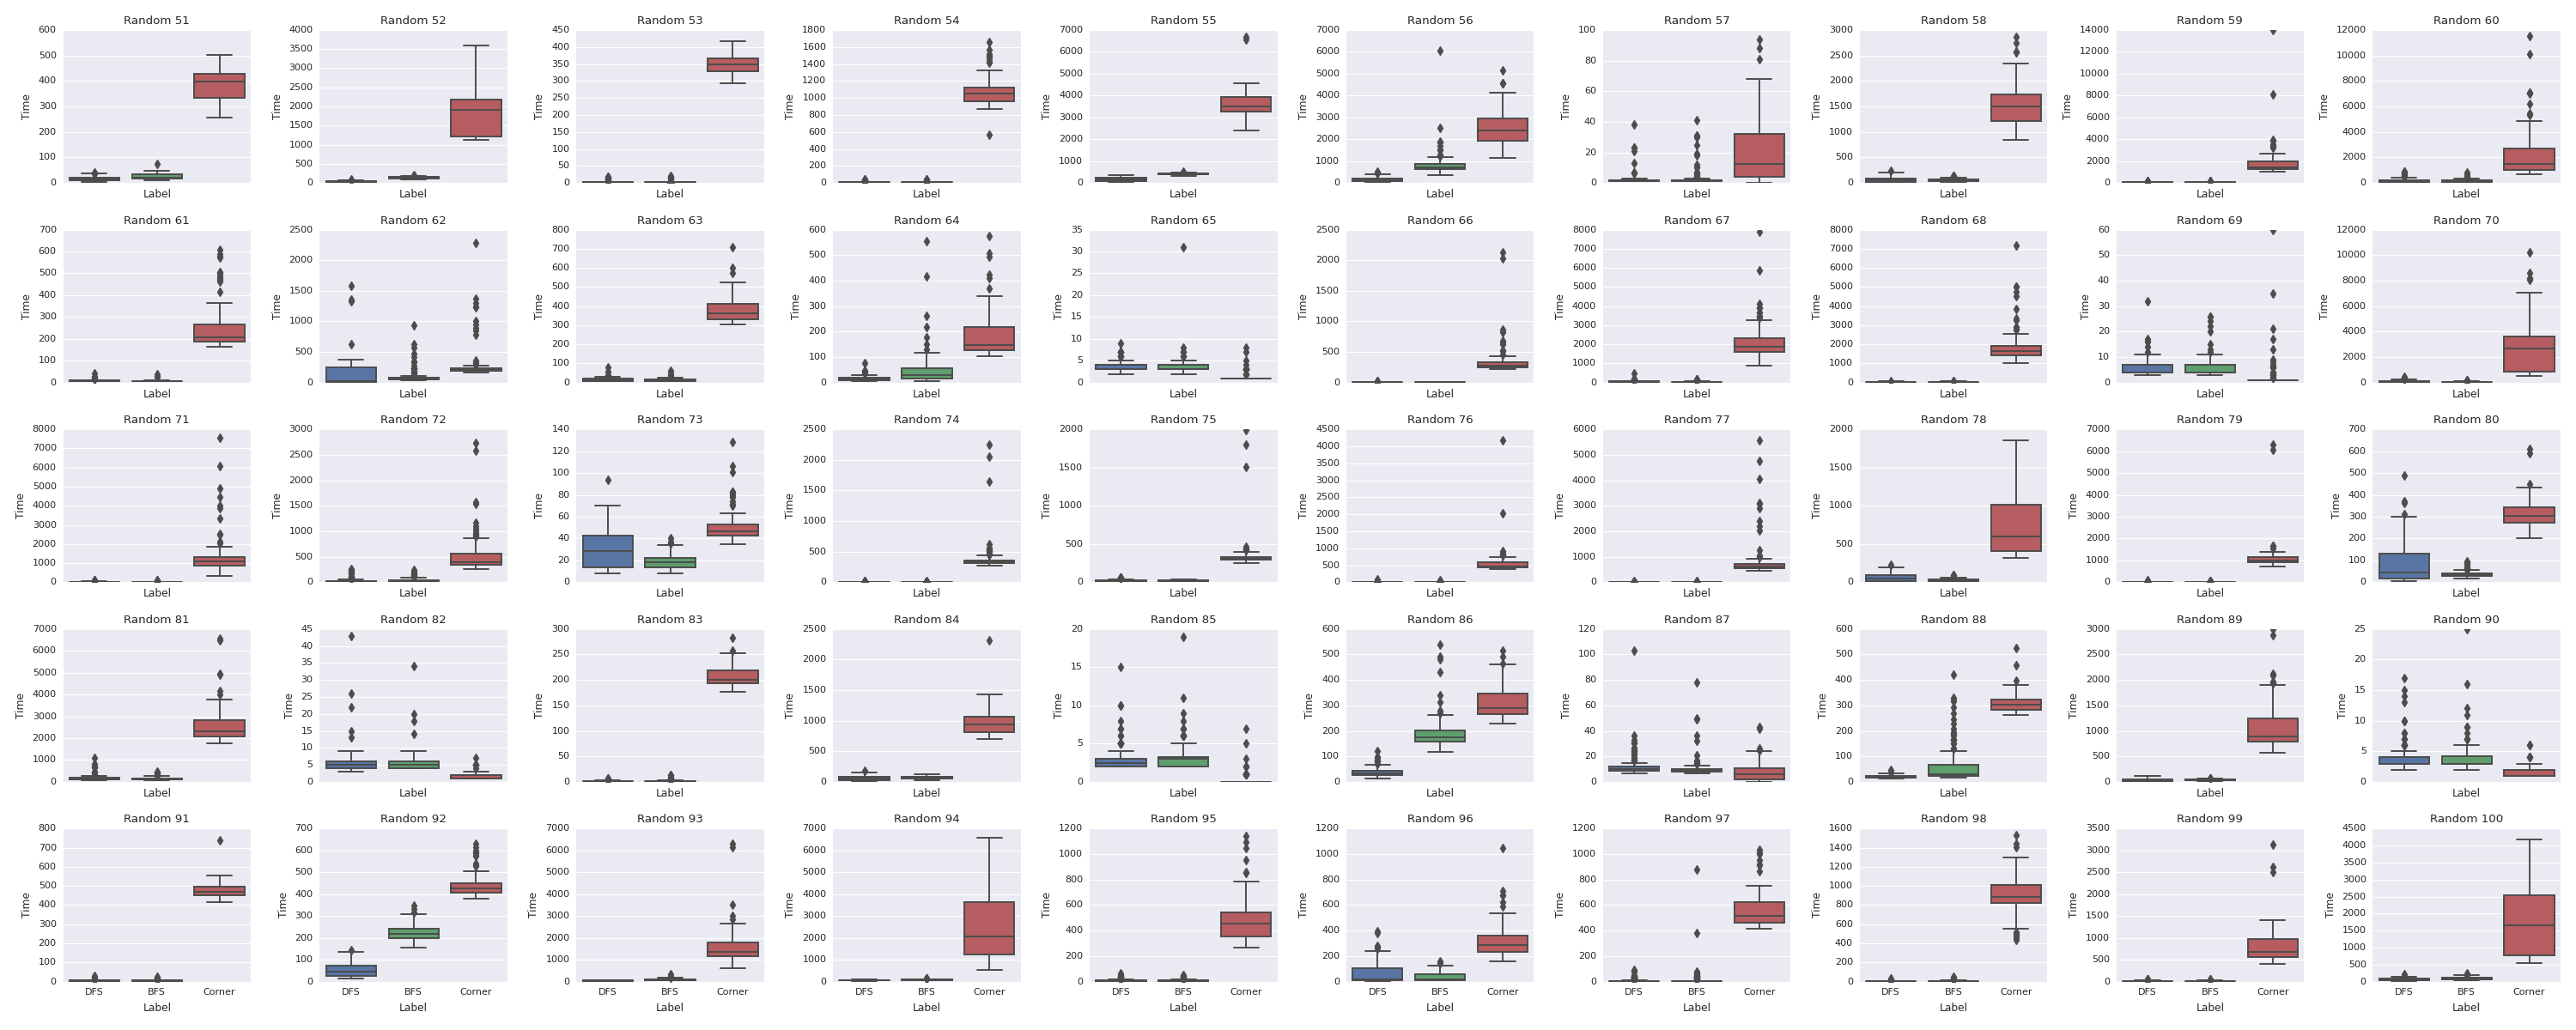
\includegraphics[width=1\linewidth]{Random50-99.png} 
\caption{The results of Experiments 51-100 of the Random experiments.}
\end{figure} 

\begin{figure}[htbp]
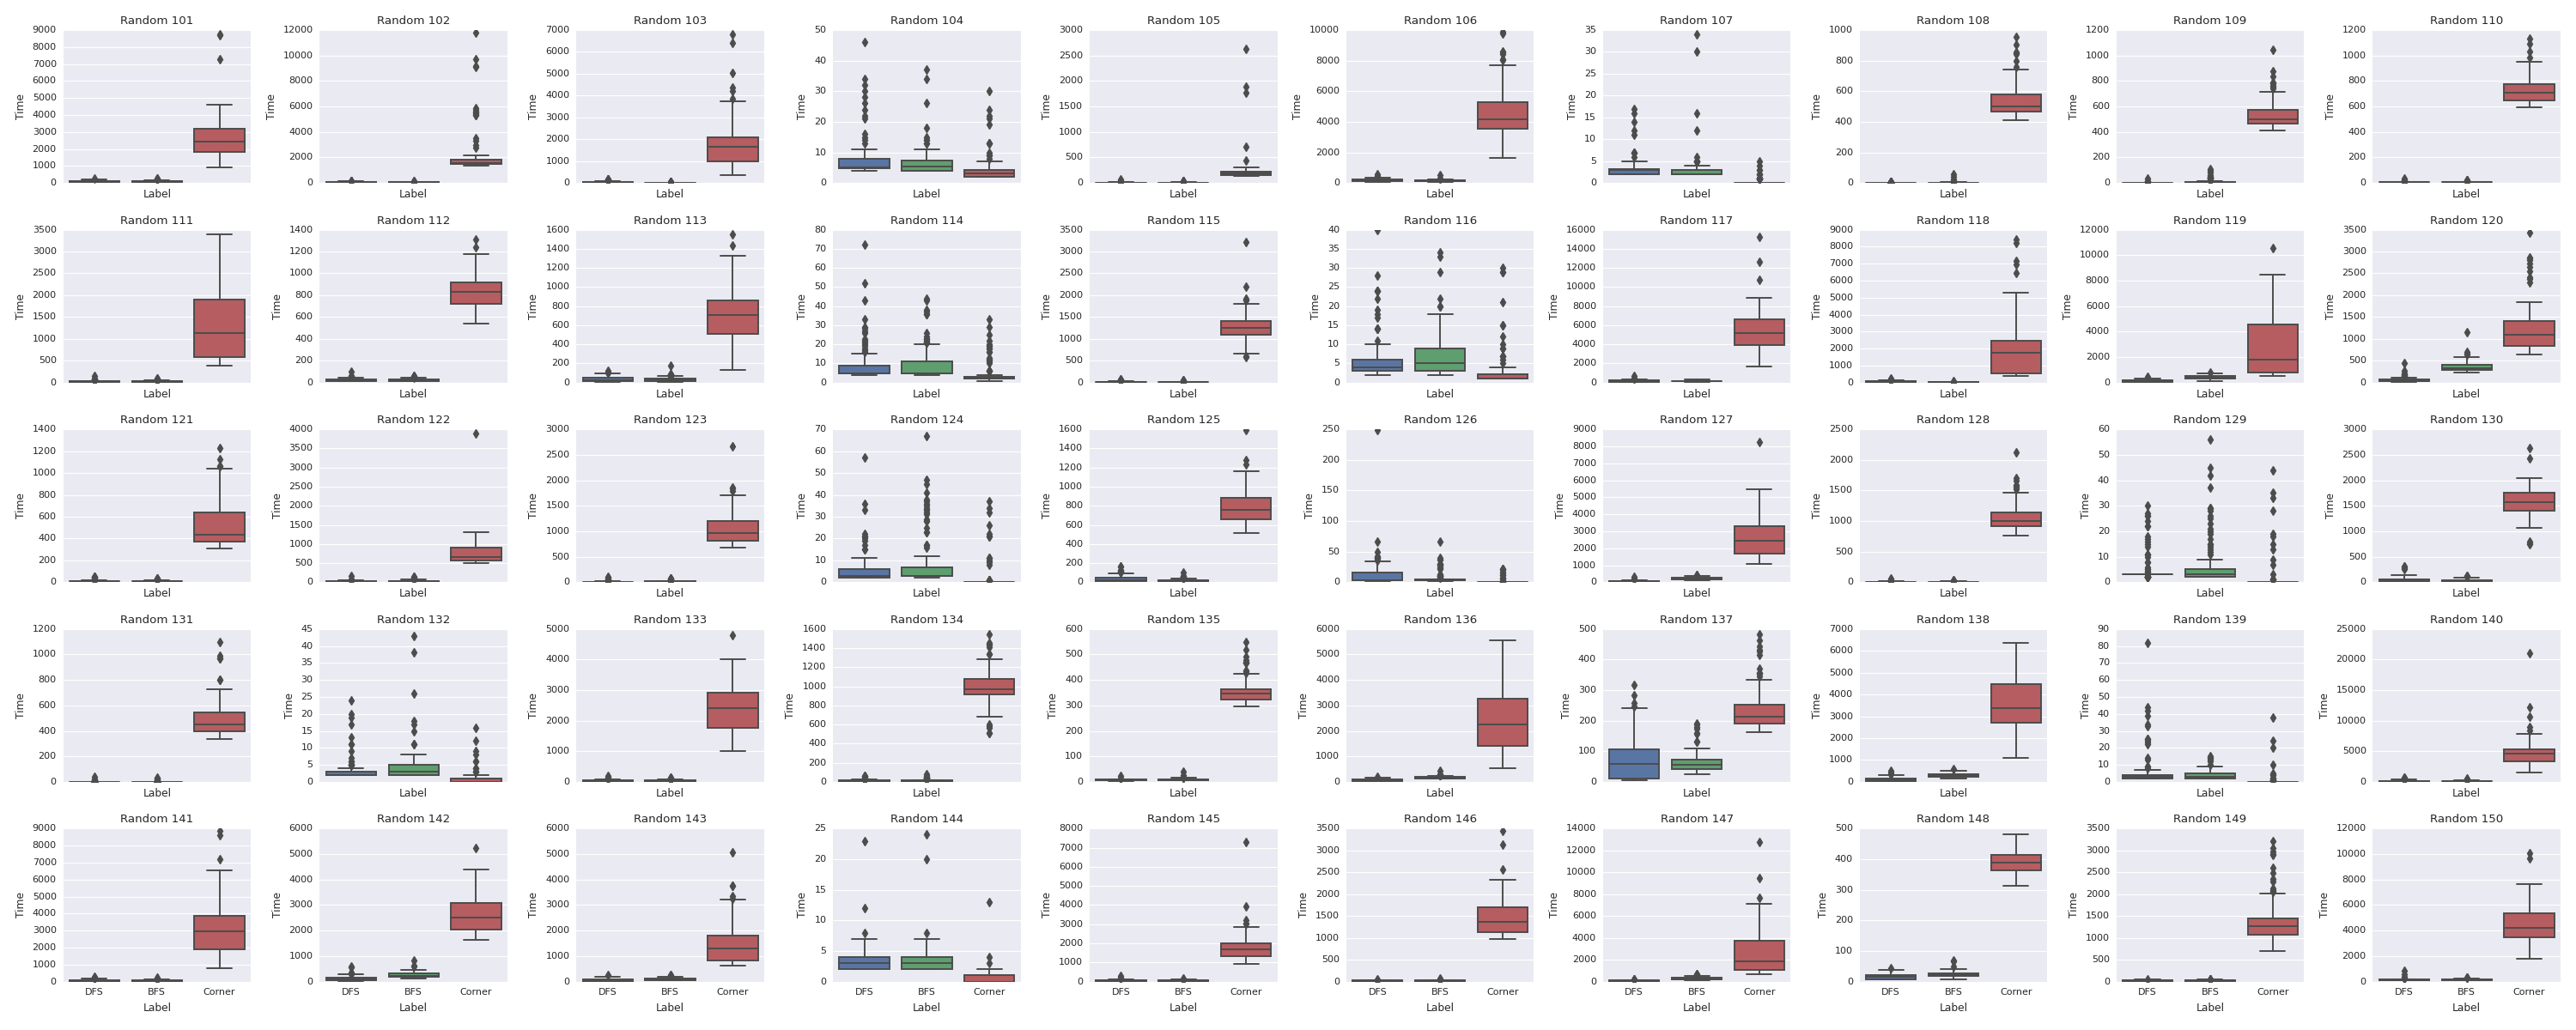
\includegraphics[width=1\linewidth]{Random100-149.png} 
\caption{The results of Experiments 101-150 of the Random experiments.}
\end{figure} 

\begin{figure}[htbp]
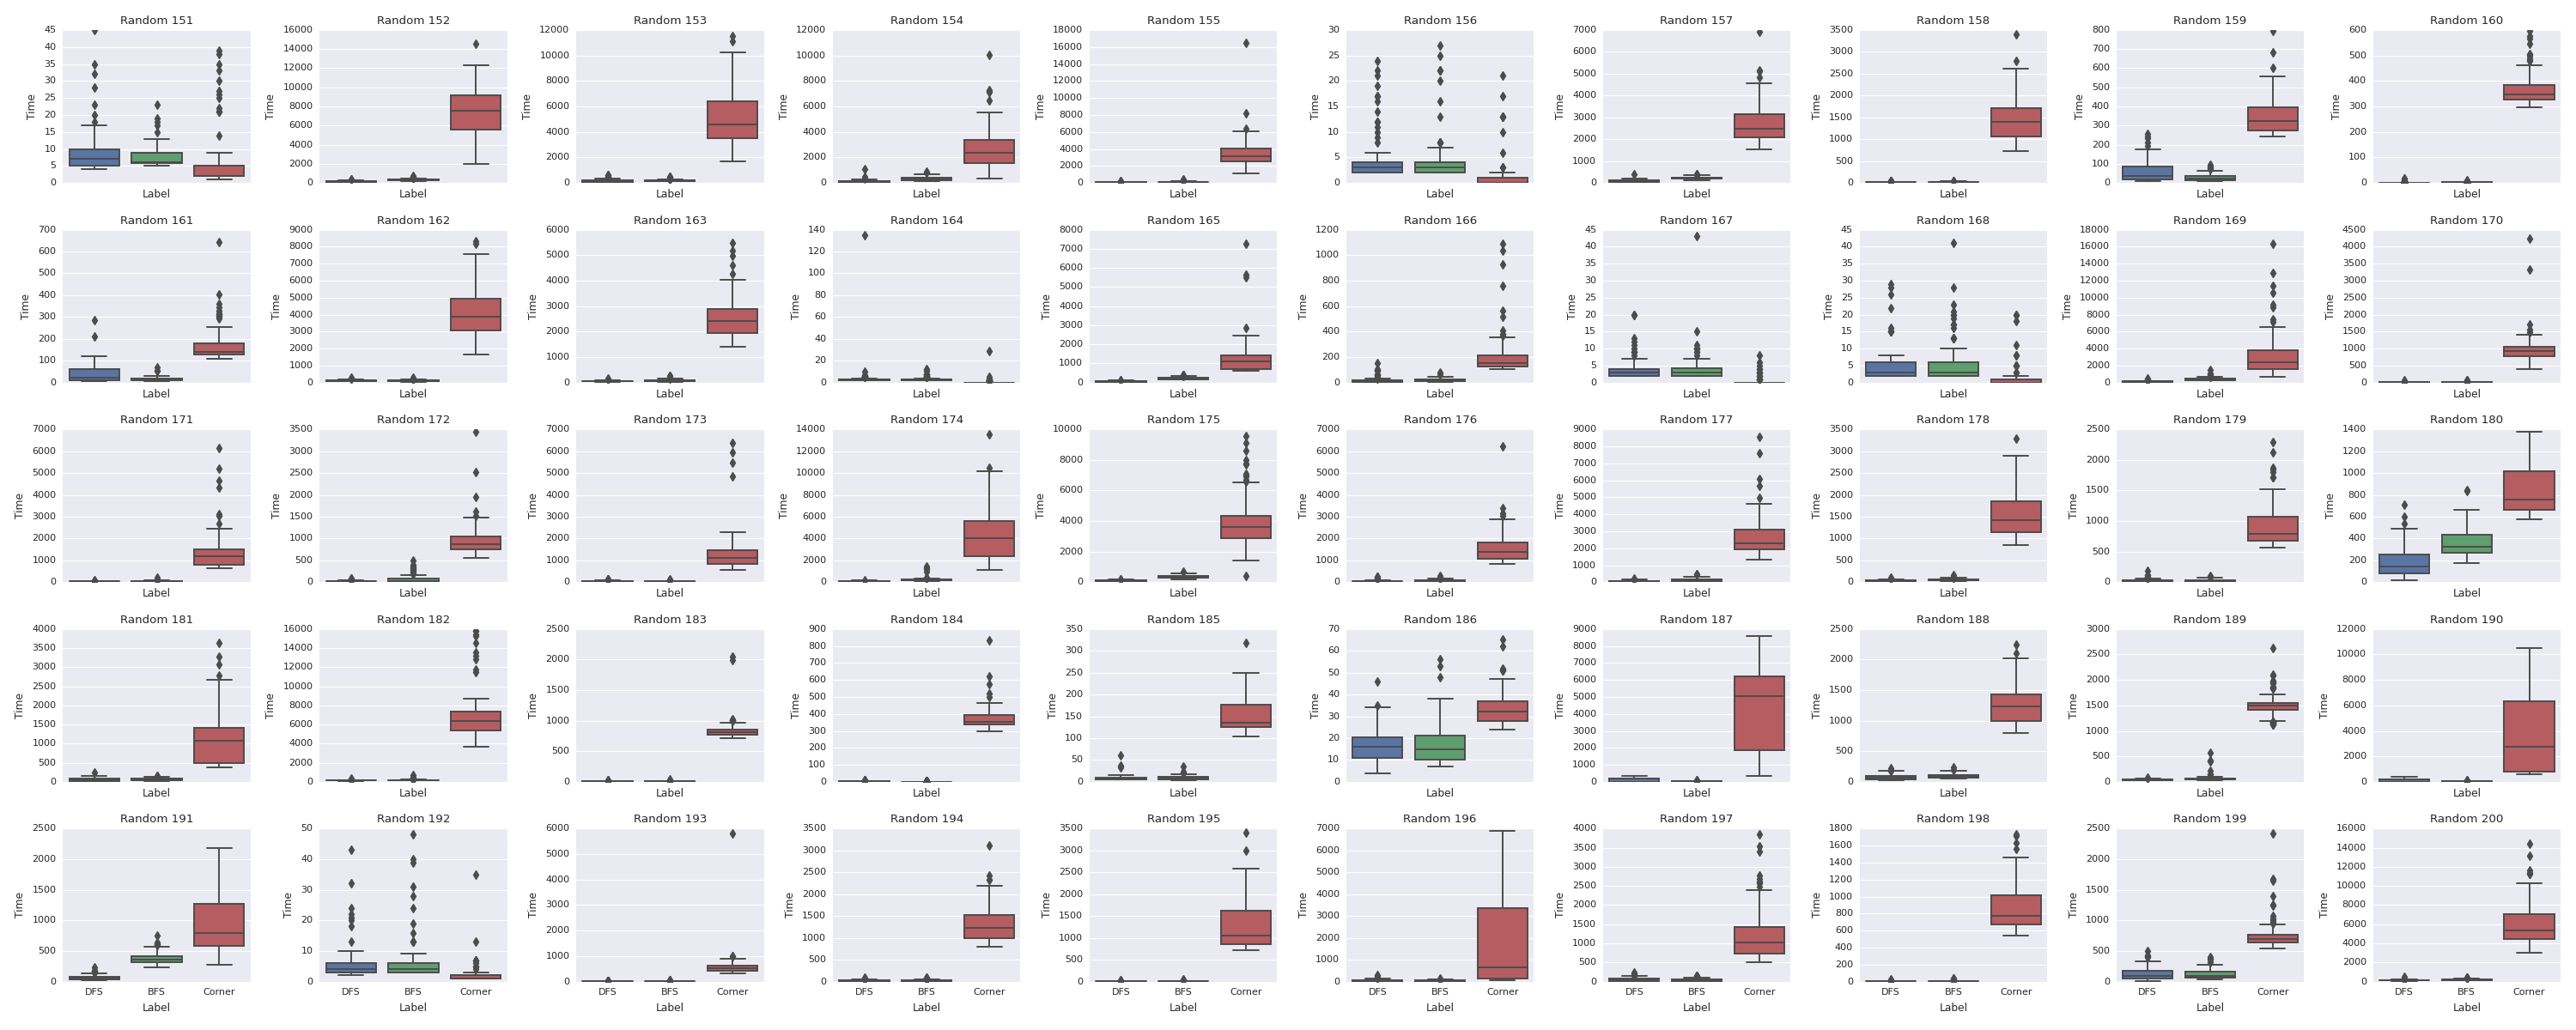
\includegraphics[width=1\linewidth]{Random150-199.png} 
\caption{The results of Experiments 151-200 of the Random experiments.}
\end{figure} 

\begin{figure}[htbp]
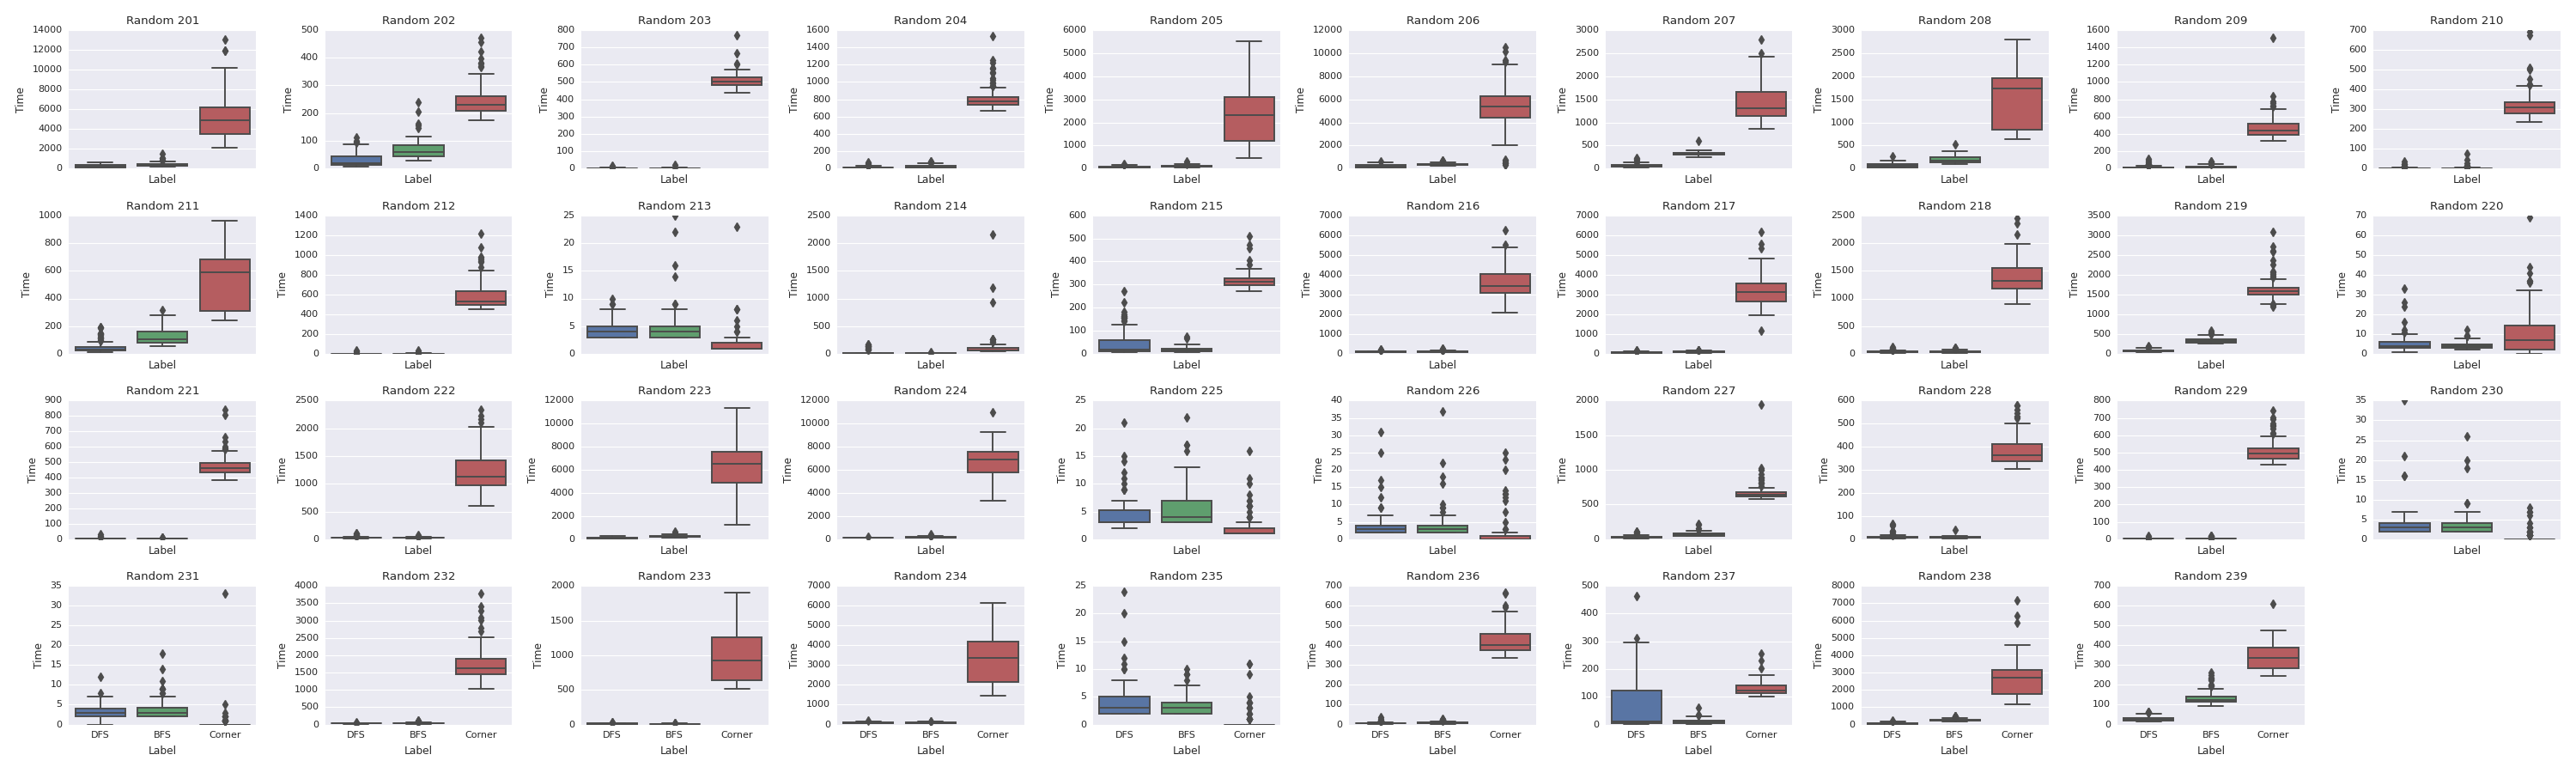
\includegraphics[width=1\linewidth]{Random200-238.png} 
\caption{The results of Experiments 201-239 of the Random experiments.}
\end{figure} 

On average the Corner- and Room-Based Model takes longer than either of the Graph-Based Models, and this intuition is played out in the results. Of the $ 219 $ Algorithm experiments, the Modified DFS Model has the lowest average execution time $ 132 $ times, the Modified BFS Model has the lowest average time $ 49 $ times, and the Corner- and Room-Based Model has the lowest average time $ 38 $ times. Of the $ 239 $ Random experiments, the Modified DFS Model has the lowest average time $ 125 $ times, the Modified BFS Model has the lowest average time $ 78 $ times, and the Corner- and Room-Based Model has the lowest average time $ 36 $ times. We can see this data in \textbf{Table 1} and \textbf{Table 2}. Interestingly, the Modified BFS Model seems to do better in the Random experiments; more work is required to identify the cause of this discrepancy. 

\begin{table}
\caption{Algorithm Experiments - Number of Times Each Model is ``Best''}
\centering
\begin{tabular}{|c|c|c|l|} \hline
Model&Number Tests With Lowest Average Time&Percentage\\ \hline
DFS&$ 125 $&$ 52.30\% $\\ \hline
BFS&$ 78 $&$ 32.64\% $\\ \hline
C- \& R-Based&$ 36 $&$ 15.06\% $\\ \hline
\end{tabular}
\end{table}

\begin{table}
\caption{Random Experiments - Number of Times Each Model is ``Best''}
\centering
\begin{tabular}{|c|c|c|l|} \hline
Model&Number Tests With Lowest Average Time&Percentage\\ \hline
DFS&$ 132 $&$ 60.27\% $\\ \hline
BFS&$ 49 $&$ 22.37\% $\\ \hline
C- \& R-Based&$ 38 $&$ 17.35\% $\\ \hline
\end{tabular}
\end{table}

We also plot all the times taken by each model into a histogram. Here, we have chosen to separate between successful and failed maps\footnote{Our hypothesis that the Random algorithm would produce more unsuccessful maps turned out true, as the Random process produced $ 85 \ (35.56\%) $ failed maps, and the Algorithm process produced $ 6 \ (0.03\%) $ failed maps.}, which allows us to examine which model catches failure the quickest. We have plotted these results in \textbf{Figure 16} through \textbf{Figure 19}. Even though comparing across maps does not tell the complete story due to discrepancies in scarcity and the distance between the hider and the seeker at the start, it does allow us to get a fairly good overall picture of the data. We see that the Corner- and Room-Based model does seem to take longer on both successful and failed maps. The reasons for this outcome are explained in \textbf{Section \ref{Discussion}}\footnote{Note that the actual means do confirm this intuition. On average for successful runs on the Algorithm maps, the DFS model takes $ 87.90 $ milliseconds, the BFS model takes $ 157.05 $ milliseconds, and the Corner- and Room-Based Model takes $ 1713.51 $ milliseconds. For failed runs on the Algorithm maps, these numbers are $ 186.46 $, $ 208.32 $, and $ 3110.46 $, respectively. For successful runs on the Random maps, these numbers are $ 52.65 $, $ 103.99 $, and $ 1262.31 $, respectively, and for failed runs these numbers are $ 34.38 $, $ 36.78 $, and $ 1414.34 $, respectively.}.

\begin{figure}[htbp]
\begin{minipage}{.48\linewidth}
\centering
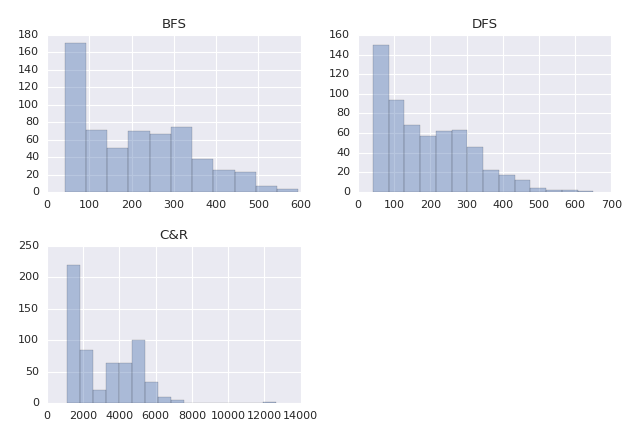
\includegraphics[width=1\linewidth]{TimeHistAlg.png} 
\end{minipage}
\begin{minipage}{.48\linewidth}
\centering
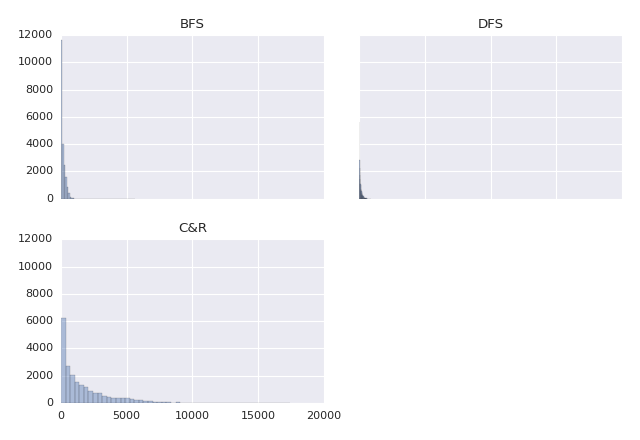
\includegraphics[width=1\linewidth]{TimeHistAlgShare.png} 
\end{minipage}
\caption{Histograms of times taken on successful runs through maps generated by the Algorithm method. The right plot shares the axes to demonstrate how the Corner- and Room-Based model does take more time.}
\end{figure} 

\begin{figure}[htbp]
\begin{minipage}{.48\linewidth}
\centering
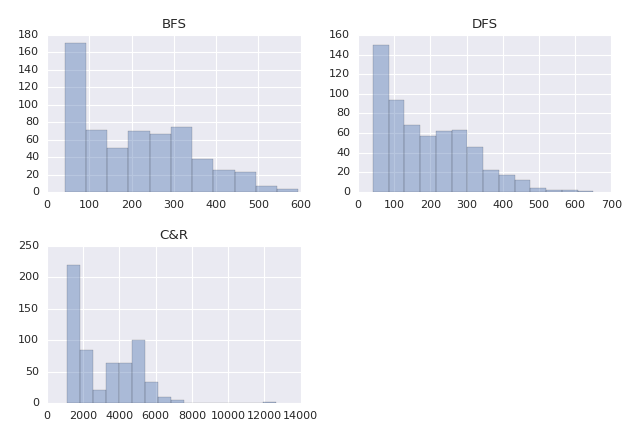
\includegraphics[width=1\linewidth]{TimeHistAlgFailed.png} 
\end{minipage}
\begin{minipage}{.48\linewidth}
\centering
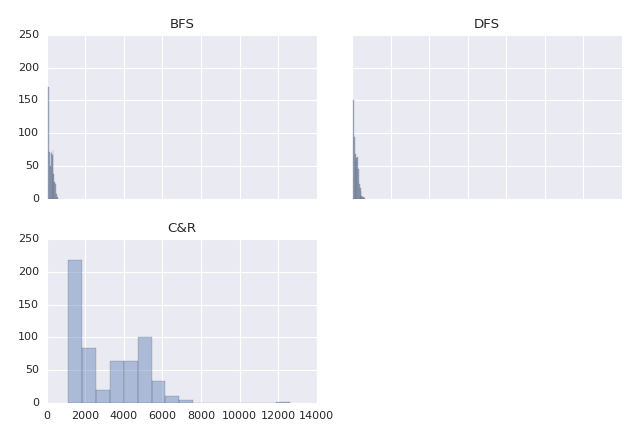
\includegraphics[width=1\linewidth]{TimeHistAlgFailedShare.png} 
\end{minipage}
\caption{Histograms of times taken on failed runs through maps generated by the Algorithm method. The right plot shares the axes to demonstrate how the Corner- and Room-Based model does take more time.}
\end{figure} 

\begin{figure}[htbp]
\begin{minipage}{.48\linewidth}
\centering
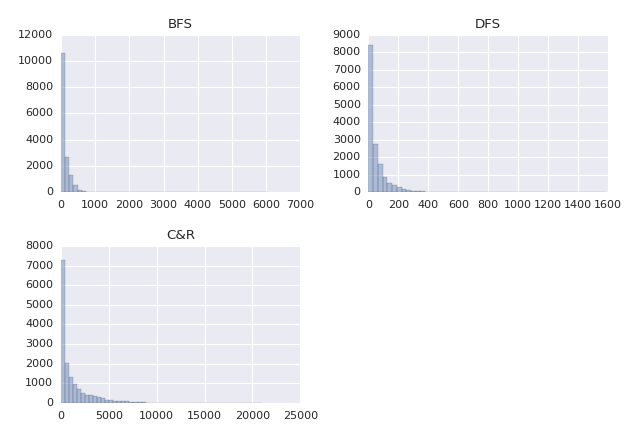
\includegraphics[width=1\linewidth]{TimeHistRandom.png} 
\end{minipage}
\begin{minipage}{.48\linewidth}
\centering
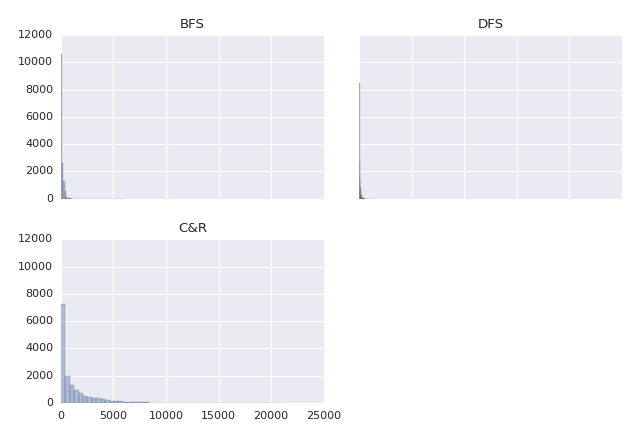
\includegraphics[width=1\linewidth]{TimeHistRandomShare.png} 
\end{minipage}
\caption{Histograms of times taken on successful runs through maps generated by the Random method. The right plot shares the axes to demonstrate how the Corner- and Room-Based model does take more time.}
\end{figure} 

\begin{figure}[htbp]
\begin{minipage}{.48\linewidth}
\centering
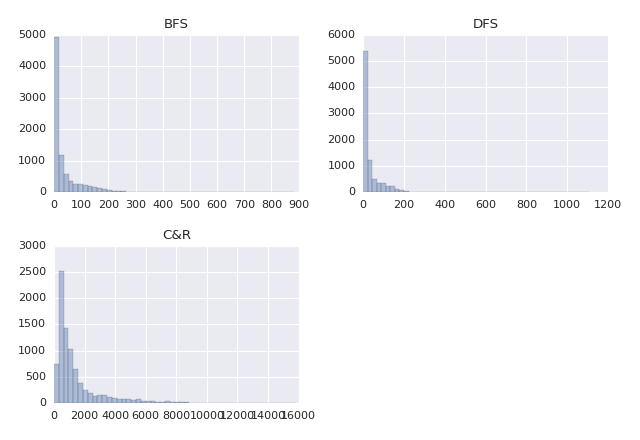
\includegraphics[width=1\linewidth]{TimeHistRandomFailed.png} 
\end{minipage}
\begin{minipage}{.48\linewidth}
\centering
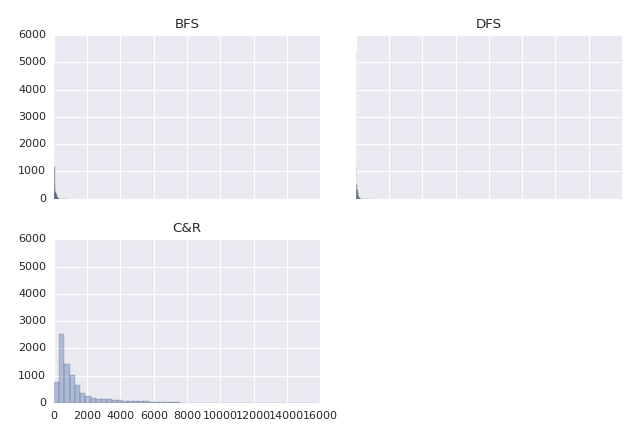
\includegraphics[width=1\linewidth]{TimeHistRandomFailedShare.png} 
\end{minipage}
\caption{Histograms of times taken on failed runs through maps generated by the Random method. The right plot shares the axes to demonstrate how the Corner- and Room-Based model does take more time.}
\end{figure} 

Furthermore, we see in \textbf{Figure 20} and \textbf{Figure 21} that, as we might assume, scarcities towards the middle range (i.e. away from 0 or 100) produce much more variance in the times produced by each model since there are increased numbers of potential layouts and different ways to explore the map. 

\begin{figure}[htbp]
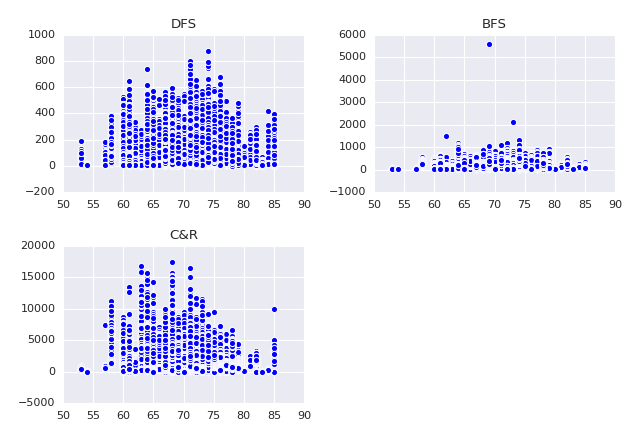
\includegraphics[width=1\linewidth]{ScarcityTimeAlg.png} 
\caption{Scatterplot of time taken on maps of different scarcity produced by the Algorithm method.}
\end{figure} 

\begin{figure}[htbp]
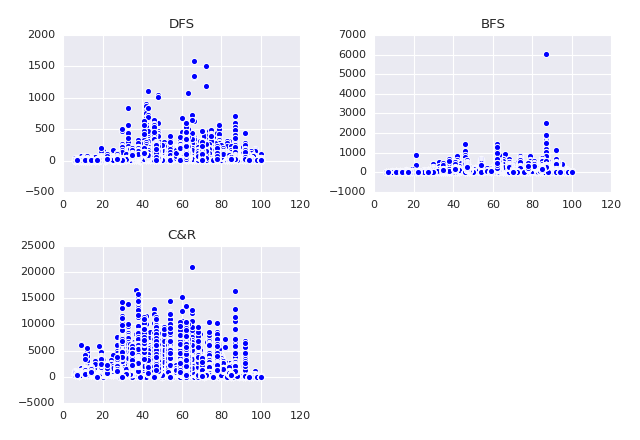
\includegraphics[width=1\linewidth]{ScarcityTimeRandom.png} 
\caption{Scatterplot of time taken on maps of different scarcity produced by the Random method.}
\end{figure} 

Interestingly, as \textbf{Figure 22} and \textbf{Figure 23} show, the BFS model produces much more consistent runs no matter the separation between the hider and seeker at the start. More work should be done to identify the cause of its consistency. 

\begin{figure}[htbp]
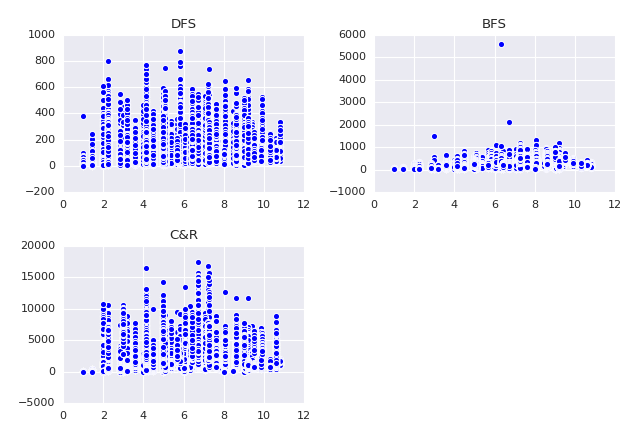
\includegraphics[width=1\linewidth]{SepTimeAlg.png} 
\caption{Scatterplot of time taken on maps of different separations produced by the Algorithm method.}
\end{figure} 

\begin{figure}[htbp]
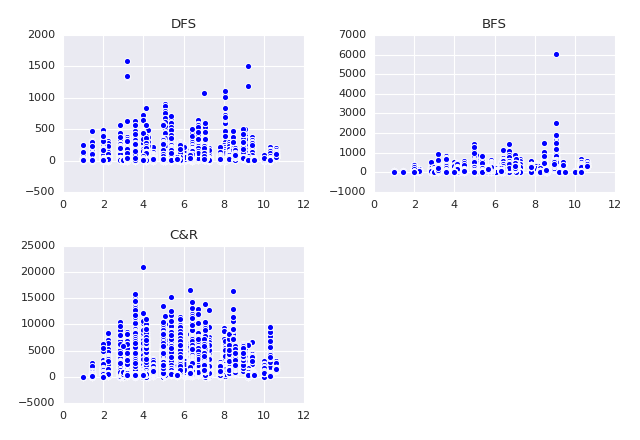
\includegraphics[width=1\linewidth]{SepTimeRandom.png} 
\caption{Scatterplot of time taken on maps of different separations produced by the Random method.}
\end{figure} 

\section{Discussion} \label{Discussion}
Using average time as a proxy for performance might lead us to wonder why we even developed the Corner- and Room-Based Model in the first place. This Model was meant to attempt to approximate human-like behavior. When looking for a hider in Hide-and-Seek, we know that if we have searched an entire room we need not go back to it and that looking around corners leads us to new places to explore.

I hypothesize that the large discrepancy in the timings among the various algorithms comes down to the large amount of time the Corner- and Room-Based Model takes to scan walls. If future work can use a vision cone or some other method to speed up this process, then the model might be able to lessen the gap with the others while still acting somewhat similar to a human agent. For example, on a map where the seeker is stuck in a block surrounded by walls to begin, the seeker scans all four walls surrounding it before terminating, while the Graph-Based Models almost immediately conclude that they have no possible tiles to which they can move. 

\section{Future Work}
Future work could follow several directions. It could expand the testing to bigger and better maps and test how the models react and scale (e.g. does the memory usage of these models hold up under bigger conditions?). It could work to adapt these models to a continuous pursuit-evasion model, with the introduction of diagonal walls and other obstacles. It could introduce an intelligent hider, which attempts to avoid the seeker. All the models as implemented in this paper will break if the hider moves since they try to never return to an explored block. Care should also be given to make sure that the performance of the various models is not based on randomly stumbling into the hider and instead based on actually finding the hiding place. The aforementioned research laid out in the Introduction should aid in this expansion. 

\appendix
\appendixpage

\section{Code}
The code used in this project can be found on GitHub at \url{https://github.com/tas12740/Seeking}.

\bibliography{sigkddExp}
\bibliographystyle{abbrv}


\end{document}
